\documentclass[10pt,brazil]{beamer}
\usepackage[T1]{fontenc}
\usepackage{lmodern}
\usepackage[utf8]{inputenc}
\usepackage[brazil]{babel}
\ifdefined\shownotes
    \usepackage{pgfpages}
    \setbeameroption{show notes on second screen=right}
\fi
\usepackage{color,colortbl,multirow}
\usetheme{Luebeck}
\useoutertheme{infolines}
\usepackage{xcolor}
\usepackage{colortbl}
\usepackage{wasysym}
\usepackage{tikz}
\usetikzlibrary{shapes.geometric,arrows.meta,positioning}
\usepackage{ragged2e}
\usepackage{caption}
\definecolor{azul}{HTML}{962038}
\setbeamercolor{structure}{fg=azul}
\setbeamertemplate{navigation symbols}{}
\usepackage{multicol}
\usepackage{algorithm} 
\usepackage{algpseudocode} 
\usepackage{bibentry}
\usepackage{graphicx}

\usepackage[alf]{abntex2cite}

\pgfdeclareimage[height=1.8cm]{logo}{img/UFOP}
\logo{\pgfuseimage{logo}}
\newcommand{\nologo}{\setbeamertemplate{logo}{}}
\setlength{\parskip}{0.2cm}

\title[Caracterização de Gargalos 802.11]{Caracterização de gargalos em redes 802.11 em ambientes de alta densidade: estudo de caso em WLAN universitária}

\author[Guimarães, I. C.]{Igor Carvalho Guimarães \\~\\  \textbf{Professor Orientador}: Marlon Paolo Lima \\ \textbf{Professor Coorientador}: Plínio Roque de Almeida} 

\institute[ICEA - UFOP]{ICEA -- Universidade Federal de Ouro Preto}
\date{2026}

\begin{document}
    \maketitle
    \note{
        [~1 min] BOM DIA / BOA TARDE à banca. \\
        Meu nome é Igor Carvalho Guimarães. \\
        Apresento meu TCC: ``Caracterização de gargalos em redes 802.11 em ambientes de alta densidade''. \\
        Orientador: Prof. Marlon Paolo Lima. Coorientador: Prof. Plínio Roque de Almeida.
    }
    
    \begin{frame}{Sumário}
        \tableofcontents
	\end{frame}
    \note{
        [~30 seg] Estrutura da apresentação: \\
        1. Introdução e contextualização da WLAN do ICEA. \\
        2. Motivação e objetivos do estudo. \\
        3. Metodologia de coleta, processamento e classificação. \\
        4. Resultados (estatística, correlações, testes, clusters). \\
        5. Recomendações práticas e conclusões.
    }

    \section{Introdução}
	\begin{frame}{Introdução}{Cenário do Campus e Infraestrutura de Rede}	
        \begin{itemize}
            \item \textbf{Cenário de Operação}: Campus do ICEA/UFOP em João Monlevade, atendendo uma comunidade de cerca de \textbf{2.500 usuários ativos} (estudantes, professores e técnicos).
            \item \textbf{Conectividade Externa (Backbone)}: \textbf{Link dedicado Full-Duplex de 1 Gbps fornecido pela RNP} (Rede Nacional de Ensino e Pesquisa), gerenciado por firewall pfSense.
            \item \textbf{Infraestrutura Sem Fio Heterogênea (40 APs no total)}:
            \begin{itemize}
                \item \textbf{23 APs Ruckus ZoneFlex R600} (MIMO 3x3:3, dual-band 2,4 GHz e 5 GHz com antenas dinâmicas BeamFlex) cobrindo salas de aula, laboratórios e biblioteca.
                \item \textbf{17 APs UniFi legados} (modelos BZ2/p2N, operação observada em 2,4 GHz) cobrindo gabinetes docentes e áreas administrativas.
            \end{itemize}
            \item \textbf{Demanda Real e Escala}: Picos simultâneos superiores a \textbf{500 clientes ativos} concorrendo no mesmo meio aéreo.
        \end{itemize} 
    \end{frame}
    \note{
        [~1,5 min] Contextualizar o cenário real onde o estudo foi desenvolvido: \\
        O campus do ICEA em João Monlevade abriga cerca de 2.500 usuários regulares. \\
        A conectividade de internet NÃO é discada nem fraca: temos um link corporativo robusto de 1 Gbps full da RNP. \\
        A rede sem fio conta com exatamente 40 Pontos de Acesso: 23 Ruckus de alto padrão em áreas de alunos e 17 UniFi legados em gabinetes. \\
        Nos horários de pico letivo, mais de 500 dispositivos móveis conectam-se simultaneamente.
    }
   
    \begin{frame}{Introdução}{O Problema Real de Pesquisa}	
        \begin{block}{A Queixa do Usuário vs. A Visibilidade da Gestão}
            Estudantes e docentes relatam frequentemente lentidão e quedas de conexão. Contudo, a equipe de TI carece de métricas quantitativas unificadas para isolar a causa raiz.
        \end{block}
        \begin{itemize}
            \item \textbf{O Mito do Cabeamento}: É comum culpar o link de internet (1 Gbps) ou a infraestrutura de rede local, quando o verdadeiro gargalo reside na física do meio sem fio.
            \item \textbf{O Desafio da Heterogeneidade}: Ruckus (SmartZone SNMP) e UniFi (HTTP API) operam no mesmo espaço físico, mas com métricas e frequências de amostragem incompatíveis.
            \item \textbf{A Pergunta Central}: \textit{Onde realmente ocorrem os gargalos (sinal fraco, congestionamento de canal, interferência, roaming instável ou saturação de cabo) e como diagnosticá-los de forma empírica?}
        \end{itemize}
	\end{frame}
    \note{
        [~1 min] Este slide apresenta o cerne do problema científico e prático: \\
        A insatisfação dos alunos com o Wi-Fi é real, mas quase sempre atribuída genericamente à 'internet da faculdade'. \\
        Como provar se o problema é o link da RNP, o cabeamento, a falta de APs ou a física do rádio? \\
        Sem dados unificados de telemetria, a tomada de decisão é cega. Esse trabalho foi desenvolvido exatamente para responder com precisão onde residem os gargalos reais do campus.
    }
	    
    \section{Motivação e Objetivos}
    \begin{frame}{Motivação}
        \begin{itemize}
            \item \textbf{Desafio da Alta Densidade}: Práticas de radiofrequência mostram que muitos clientes ativos degradam severamente o tempo aéreo comum (\textit{airtime}) \cite{gast2005}.
            \item \textbf{Obsolescência e Heterogeneidade}: Equipamentos corporativos de ponta (Ruckus R600) coexistindo com redes mais simples (UniFi) sem coordenação de RF.
            \item \textbf{Percepção do Usuário}: Frequente insatisfação com a estabilidade e velocidade da conexão de rede corporativa, necessitando de um diagnóstico livre de viés qualitativo puramente opinativo.
            \item \textbf{Ociosidade vs. Abuso}: Falta de visibilidade técnica sobre o uso abusivo de banda por poucos usuários limitando a estabilidade geral dos demais.
        \end{itemize}
    \end{frame}
    \note{
        [~1,5 min] CSMA/CA: o Wi-Fi é um meio compartilhado. Cada dispositivo ativo reduz a fatia de airtime dos outros. \\
        Ruckus R600 usa BeamFlex (direcionamento dinâmico de feixe) --- vantagem física real sobre antenas omnidirecionais. \\
        Ponto político: a insatisfação dos alunos é real, mas nunca tinha sido quantificada com dados de produção. Esse trabalho faz isso.
    }
    
    \begin{frame}{Objetivos}
        \begin{block}{Objetivo Geral}
            Caracterizar e diagnosticar os gargalos físicos e lógicos que limitam o desempenho e a qualidade de experiência nas redes sem fio corporativas do ICEA/UFOP.
        \end{block}
        \begin{block}{Objetivos Específicos}
            \begin{itemize}
                \item Coleta automatizada de dados quantitativos de telemetria das controladoras (SmartZone e UniFi Controller).
                \item Pré-processamento, limpeza, unificação e padronização das métricas.
                \item Modelagem heurística determinística de classificação de gargalos.
                \item Aplicação de agrupamento não-supervisionado (\textit{K-Means}) para validação.
                \item Elaboração de sugestões e recomendações práticas de QoS e gerenciamento de RF.
            \end{itemize}
        \end{block}
    \end{frame}
    \note{
        [~1 min] Objetivo GERAL: caracterizar e diagnosticar --- não apenas descrever, mas propor soluções. \\
        Específicos: a sequência lógica vai de coleta → padronização → classificação heurística → validação K-Means → recomendações. \\
        Se a banca perguntar por que usar K-Means: porque valida os limiares heurísticos SEM supervisão, eliminando viés manual.
    }

    \section{Metodologia}
    \begin{frame}{Metodologia}{Coleta e Arquitetura de Fluxo de Dados}
        \begin{itemize}
            \item \textbf{Estudo de Caso}: Monitoramento das redes corporativas do campus (Eduroam e ICEA-WIFI).
            \item \textbf{Automação em Python 3}: Coletas diárias das controladoras via SNMP (Ruckus) e REST API (UniFi).
            \item \textbf{Período Amostral (20 Dias Úteis com Aulas Ativas)}:
            \begin{itemize}
                \scriptsize
                \item \textbf{Fase 1 (Fechamento 2026/1 -- 23/06 a 03/07)}: Fim de semestre e exames finais (máxima densidade).
                \item \textbf{Recesso Acadêmico}: Interrupção entre semestres letivos.
                \item \textbf{Fase 2 (Abertura 2026/2 -- 24/08 a 04/09)}: Retomada letiva e rotina acadêmica presencial.
            \end{itemize}
            \item \textbf{Volume Consolidado}: \textbf{498.034 registros telemétricos} reais de produção.
        \end{itemize}
        
        \begin{table}[h]
            \centering\footnotesize
            \begin{tabular}{lccc}
                \hline
                \textbf{Fabricante} & \textbf{Registros Originais} & \textbf{Registros Limpos} & \textbf{Redundância} \\
                \hline
                \textbf{Ruckus} & 446.060 & 446.060 & 0,00\% \\
                \textbf{UniFi} & 51.974 & 51.974 & 0,00\% \\
                \hline
            \end{tabular}
            \caption{Consolidação dos Datasets do Campus}
            \label{tab:resumo_coleta_slides}
        \end{table}
    \end{frame}
    \note{
        [~1,5 min] Explicar a divisão temporal dos 20 dias úteis de coleta: \\
        A coleta não foi aleatória ou em recesso; pegou dias normais de aula divididos em duas etapas letivas: \\
        1. Final do período passado (23/06 a 03/07): semanas de provas com salas cheias, onde registramos os maiores picos da Ruckus. \\
        2. Início do período atual (24/08 a 04/09): volta às aulas presenciais. \\
        Volume consolidado: quase meio milhão de registros (446 mil Ruckus e 52 mil UniFi) com redundância zero.
    }

    \begin{frame}{Metodologia}{Pipeline Metodológico da Pesquisa}
        \centering
        \vspace{-0.15cm}
        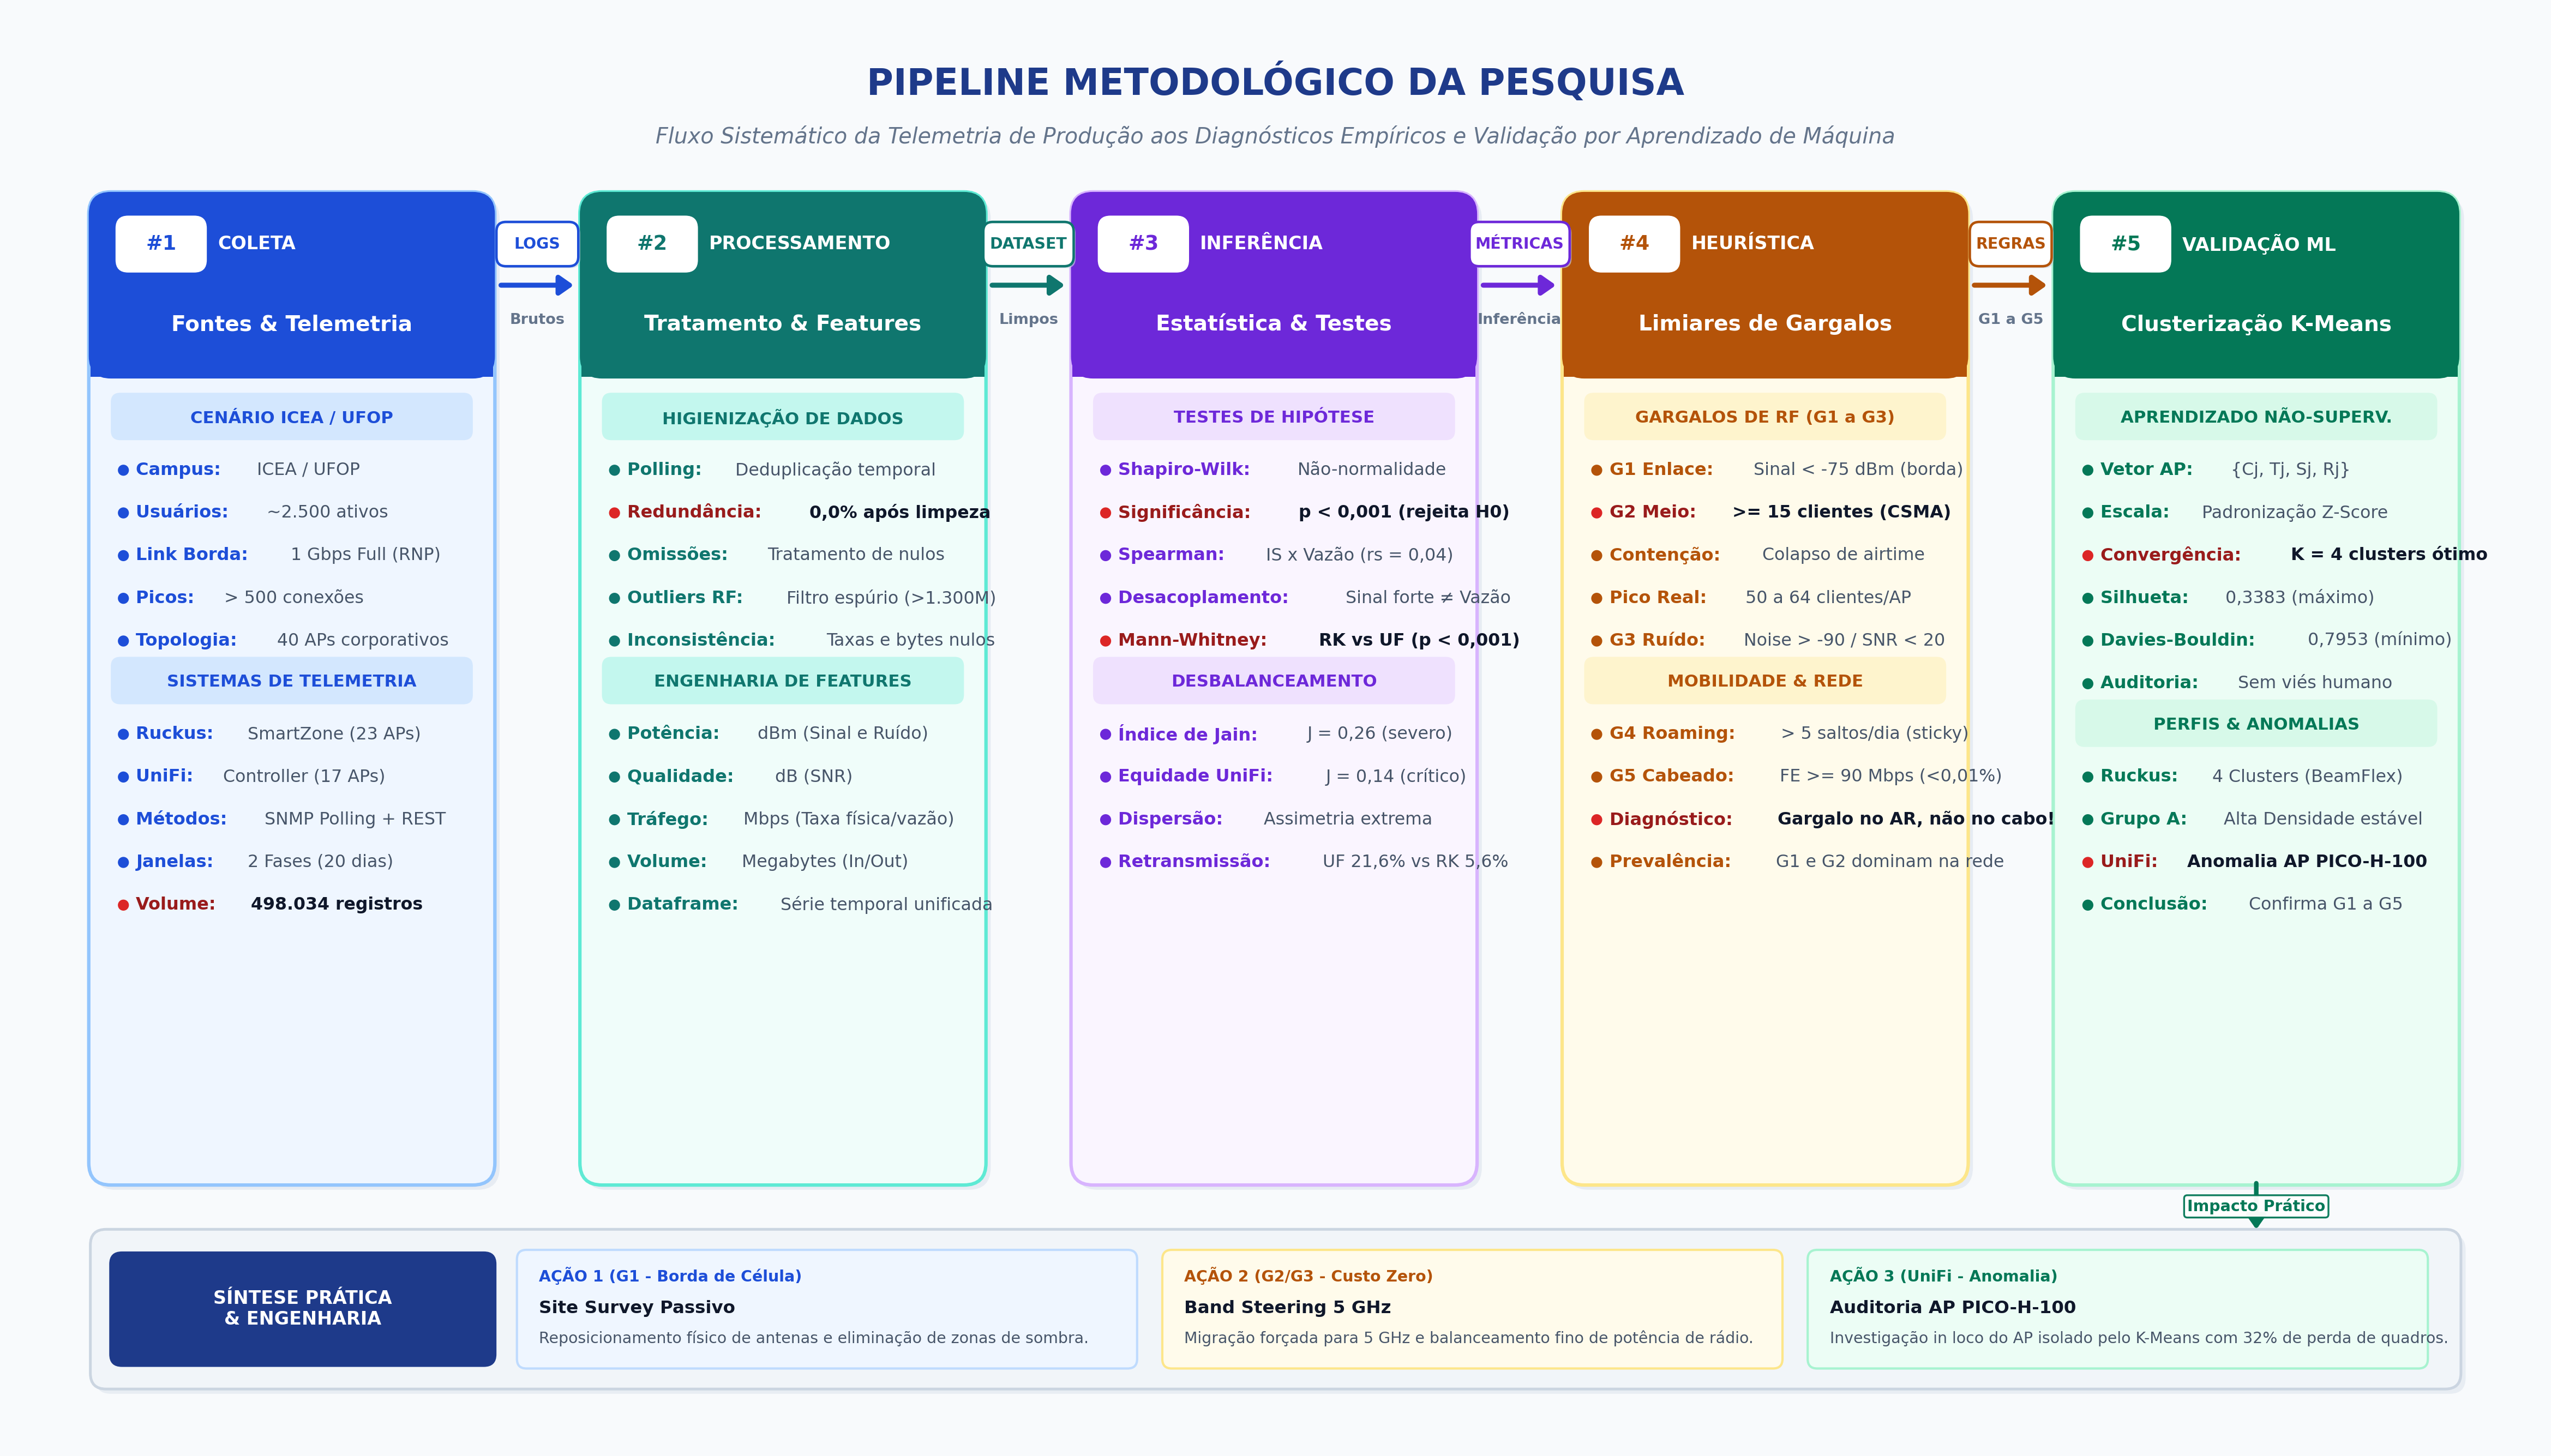
\includegraphics[width=\textwidth,height=0.82\textheight,keepaspectratio]{img/fluxograma_metodologia.png}
    \end{frame}
    \note{
        [~1,5 min] Este fluxograma sintetiza visualmente todo o pipeline metodológico construído no trabalho: \\
        1. Cenário Físico e Coleta (Etapa 1): 40 APs no ICEA, 20 dias letivos, quase meio milhão de registros via SNMP (Ruckus) e REST API (UniFi). \\
        2. Tratamento e Features (Etapa 2): deduplicação temporal (redundância zero), padronização de grandezas de RF e filtros de espúrios. \\
        3. Análise Estatística (Etapa 3): confirmação de não-normalidade (p < 0,001) e severo desbalanceamento de carga (Jain = 0,26). \\
        4. Classificação Heurística (Etapa 4): árvore determinística baseada na literatura e normas IEEE para isolar G1 a G5. \\
        5. Validação K-Means (Etapa 5): clusterização não-supervisionada que confirma matematicamente os perfis sem viés humano, fundamentando as 3 ações práticas de engenharia de redes.
    }

    \begin{frame}{Metodologia}{Limiares Determinísticos de Gargalos}
        Árvore de decisão baseada em 5 perfis heurísticos fundamentados na literatura e normas IEEE:
        \begin{itemize}
            \item \textbf{G1: Baixa Qualidade de Enlace}: Intensidade de Sinal recebida ($IS < -75$ dBm).
            \item \textbf{G2: Congestionamento do Meio}: Densidade do AP ($\ge 15$ clientes simultâneos/min).
            \begin{itemize}
                \scriptsize
                \item \textit{Fundamento CSMA/CA}: No meio compartilhado, a disputa de canal acima de 15 estações degrada severamente o tempo aéreo (\textit{airtime}) por colisões (Cisco/Ruckus High Density).
                \item \textit{Pico do Campus}: Registramos APs com \textbf{50 a 64 clientes simultâneos}.
            \end{itemize}
            \item \textbf{G3: Interferência / SNR Ruim}: Ruído permanente ($Noise > -90$ dBm) ou relação sinal-ruído marginal ($SNR < 20$ dB) sob boa IS.
            \item \textbf{G4: Instabilidade de Roaming}: Dispositivos móveis instáveis ($> 5$ transições de AP/dia).
            \item \textbf{G5: Gargalo Cabeado (Fast Ethernet)}: Saturação da interface uplink do AP ($\ge 90$ Mbps).
        \end{itemize}
    \end{frame}
    \note{
        [~1,5 min] Explicar cada gargalo com calma: \\
        Por que 15 clientes em G2? No Wi-Fi, o meio é compartilhado em half-duplex (CSMA/CA). 15 clientes disputando o mesmo canal de rádio geram severa contenção de tempo aéreo (airtime). E no campus, registramos APs com 50 a 64 clientes simultâneos nos horários de pico! \\
        G1 (-75 dBm): limiar IEEE 802.11 onde a modulação cai para MCS0 (velocidade mínima). \\
        G3 (SNR < 20 dB): ruído eletromagnético destruindo a integridade dos quadros. \\
        G4 (5 trocas/dia): celulares transitando e ficando presos a APs distantes (sticky clients). \\
        G5 (90 Mbps): teste para verificar se o problema era a porta Fast Ethernet do switch cabeado.
    }

    \section{Resultados e Discussões}
    \nologo
    \begin{frame}{Resultados}{Análise Descritiva Comparativa}
        \begin{columns}
            \begin{column}{0.50\textwidth}
                \begin{table}[h]
                    \centering
                    \resizebox{\linewidth}{!}{%
                    \begin{tabular}{llcccc}
                        \hline
                        \textbf{Fabricante} & \textbf{Métrica} & \textbf{Média} & \textbf{Q1 (25\%)} & \textbf{Mediana} & \textbf{Q3 (75\%)} \\
                        \hline
                        \textbf{Ruckus} & IS [dBm] & -73,8 & -81,0 & -75,0 & -68,0 \\
                        \textbf{UniFi}  & IS [dBm] & -66,2 & -76,0 & -67,0 & -57,0 \\
                        \hline
                        \textbf{Ruckus} & Throughput [Mbps] & 0,47 & 0,03 & 0,12 & 0,46 \\
                        \textbf{UniFi}  & Throughput [Mbps] & 0,26 & 0,00 & 0,00 & 0,02 \\
                        \hline
                        \textbf{Ruckus} & Retransm. [\%] & \textbf{5,62\%} & 0,00\% & 0,00\% & 1,59\% \\
                        \textbf{UniFi}  & Retransm. [\%] & \textbf{21,65\%} & \textbf{2,80\%} & \textbf{12,30\%} & \textbf{30,00\%} \\
                        \hline
                    \end{tabular}%
                    }
                    \caption{Estatísticas Descritivas por Quartis (Sem Outliers)}
                \end{table}
                \scriptsize
                \begin{itemize}
                    \item \textbf{Eliminação de Outliers}: Uso de quartis (Q1 e Q3) elimina leituras espúrias (ex.: $-20$ dBm a centímetros da antena).
                    \item \textbf{Vazão Mediana Ociosa}: $0,12$ Mbps (RK) e $0,00$ Mbps (UF) comprovam tráfego em segundo plano na maior parte do tempo.
                    \item \textbf{Disparidade Crítica}: UniFi opera com retransmissão mediana de \textbf{12,30\%} e Q3 de \textbf{30,00\%} (vs. 0,00\% e 1,59\% na Ruckus).
                \end{itemize}
            \end{column}
            \begin{column}{0.50\textwidth}
                \begin{figure}
                    \centering
                    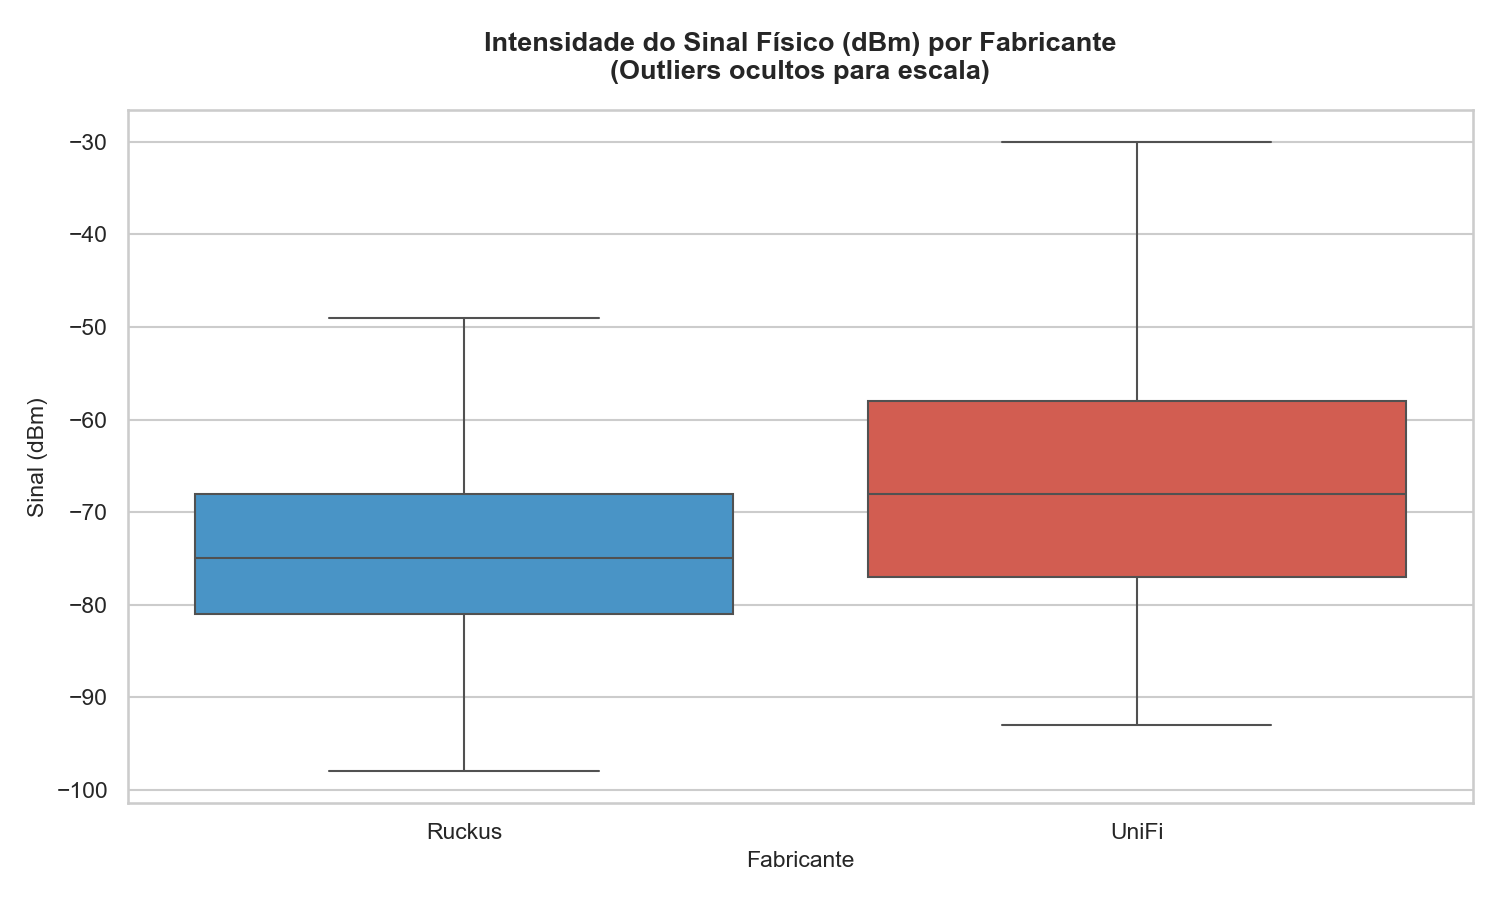
\includegraphics[width=\textwidth]{img/boxplot_rssi_fabricante.png}
                    \caption{Distribuição de Intensidade de Sinal por Fabricante}
                    \label{fig:boxplot_rssi_slide}
                \end{figure}
            \end{column}
        \end{columns}
    \end{frame}
    \note{
        \scriptsize
        \textbf{[Tempo: ~1,5 min | Roteiro de Fala - Análise Descritiva]}\\[2pt]
        $\bullet$ \textbf{Por que Quartis em vez de Máximo?} Na tabela, substituímos o valor máximo por Q1 e Q3 para eliminar \textit{outliers}. Um valor máximo de -20 dBm em Wi-Fi só ocorre se o usuário encostar o celular na carcaça do rádio (é 100 vezes mais potente que um sinal típico de -40 dBm). Os quartis mostram o miolo real da operação.\\[2pt]
        $\bullet$ \textbf{Sinal Físico (IS):} A UniFi apresenta sinal mediano ligeiramente superior (-67 dBm vs -75 dBm da Ruckus). Isso decorre da arquitetura do prédio: a UniFi está em gabinetes de professores menores, enquanto a Ruckus cobre grandes salas de aula e vãos abertos do campus.\\[2pt]
        $\bullet$ \textbf{O Grande Alarme (Retransmissões):} A UniFi opera em estado crítico. Sua mediana é de \textbf{12,30\%} e o Q3 atinge \textbf{30,00\%} de pacotes perdidos! A Ruckus opera com mediana ZERO e Q3 de apenas 1,59\% (média 5,62\% puxada por picos pontuais).\\[2pt]
        $\bullet$ \textbf{Throughput Mediano:} É próximo de zero em ambas (0,12 e 0,00 Mbps). A esmagadora maioria dos clientes conectados está apenas mantendo conexões de segundo plano (WhatsApp, notificações push).
    }

    \begin{frame}[label=slide_distribuicao]{Resultados}{Distribuição Temporal de Clientes Únicos}
        \begin{figure}
            \centering
            \hyperlink{zoom_heatmap}{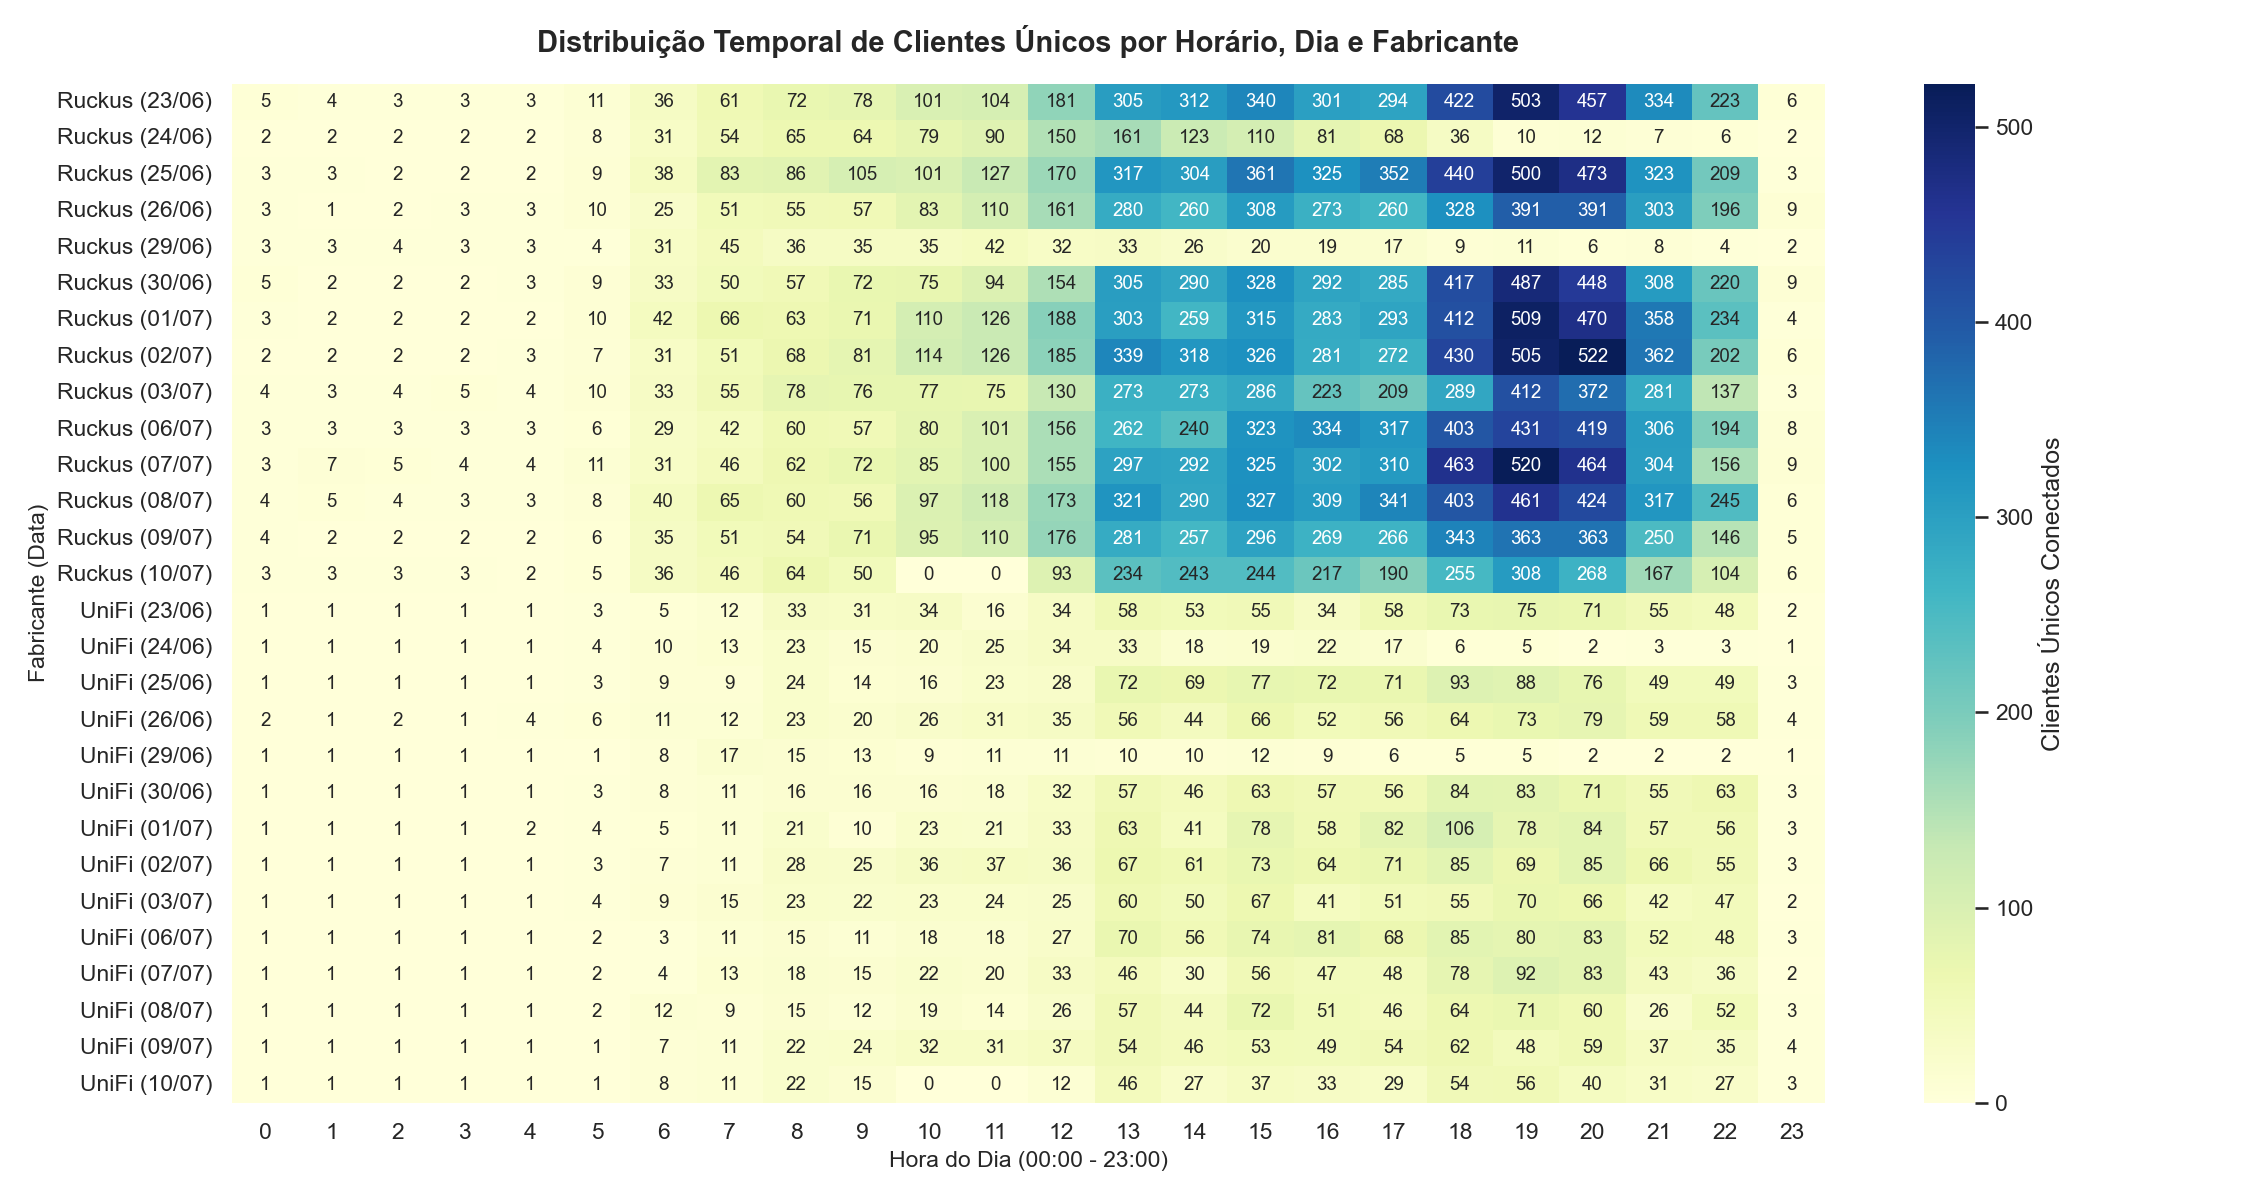
\includegraphics[width=0.88\textwidth,height=3.5cm,keepaspectratio]{img/heatmap_horario_clientes.png}}
            \caption{Distribuição de Clientes Únicos por Horário, Dia e Fabricante \quad \hyperlink{zoom_heatmap}{\beamergotobutton{Ampliar}}}
            \label{fig:heatmap_clientes_slides}
        \end{figure}
        \scriptsize
        \begin{itemize}
            \item \textbf{Janelas Letivas (20 dias)}: Fase 1 (fim de 2026/1, exames finais) e Fase 2 (início de 2026/2, retorno das aulas), intercaladas pelo recesso acadêmico de julho/agosto.
            \item \textbf{Ciclo Circadiano}: Atividade residual noturna, ascensão rápida às 08h, ápice letivo (14h--18h) e esvaziamento progressivo após 22h.
            \item \textbf{Disparidade de Carga}: Ruckus atingiu pico de \textbf{522} clientes/h (02/07 às 20h), enquanto a UniFi registrou no máximo \textbf{106} (01/07 às 18h).
            \item \textbf{Origem do Gargalo G2}: Densidade extrema nos horários de pico satura o tempo aéreo (\textit{airtime}) no protocolo de contenção CSMA/CA.
        \end{itemize}
    \end{frame}
    \note{
        \scriptsize
        \textbf{[Tempo: ~1,5 min | Roteiro de Fala - Distribuição Temporal]}\\[2pt]
        $\bullet$ \textbf{Contextualização das Janelas de Coleta:} Este mapa de calor registra 20 dias úteis divididos em duas fases reais do campus: a \textbf{Fase 1} pegou o encerramento do semestre 2026/1 com semanas de exames finais (alta permanência de alunos estudando na biblioteca e salas); houve o \textbf{recesso acadêmico}; e a \textbf{Fase 2} registrou o início de 2026/2 com a volta às aulas.\\[2pt]
        $\bullet$ \textbf{Ciclo Circadiano de 24 Horas:} A rede acompanha perfeitamente a rotina universitária: madrugada quase sem clientes, subida íngreme às 08:00 com o início das aulas matutinas, pico entre 14:00 e 18:00 e atividade contínua até 22:00.\\[2pt]
        $\bullet$ \textbf{Assimetria Visual entre as Redes:} As faixas da Ruckus operam em tons escuros e contínuos, com pico de \textbf{522 clientes únicos em uma única hora} (02/07 às 20:00). A UniFi atingiu no máximo \textbf{106 clientes} (01/07 às 18:00). Isso prova que a Ruckus sustenta a massa estudantil, enquanto a UniFi atende salas de professores e técnicos.\\[2pt]
        $\bullet$ \textbf{Origem do Gargalo G2:} Essa concentração em horários de aula explica o Gargalo G2 (44,5\% na Ruckus). Não é defeito do sinal, é colisão por disputa de tempo aéreo no CSMA/CA gerada por dezenas de aparelhos no mesmo rádio. Se quiserem ver detalhes dos dias, clique no botão \textit{Ampliar}!
    }

    \begin{frame}[label=slide_correlacoes]{Resultados}{Estudo de Correlações (Spearman)}
        \begin{columns}
            \begin{column}{0.50\textwidth}
                \scriptsize
                \begin{itemize}
                    \item \textbf{Desacoplamento Sinal x Vazão (Ruckus)}: ($r_s = 0,04$), correlação quase nula ($p < 0,001$). Ter sinal excelente não garante maior throughput na aplicação, pois o meio é fatiado via CSMA/CA \cite{bianchi2000}.
                    \item \textbf{Densidade x Throughput Agregado}: ($r_s = 0,79$ RK / $r_s = 0,53$ UF), provando que o tráfego total do AP escala consistentemente com a quantidade de clientes.
                    \item \textbf{Densidade x Retransmissões}: ($r_s = 0,35$ RK / $r_s = 0,21$ UF), confirmando matematicamente o aumento de colisões e disputa de \textit{airtime} sob adensamento.
                    \item \textbf{Ruído x Retransmissões (Ruckus)}: ($r_s = -0,64$), refletindo a sensibilidade da modulação adaptativa ao piso de ruído do canal.
                \end{itemize}
            \end{column}
            \begin{column}{0.50\textwidth}
                \begin{figure}
                    \centering
                    \hyperlink{zoom_correlacoes}{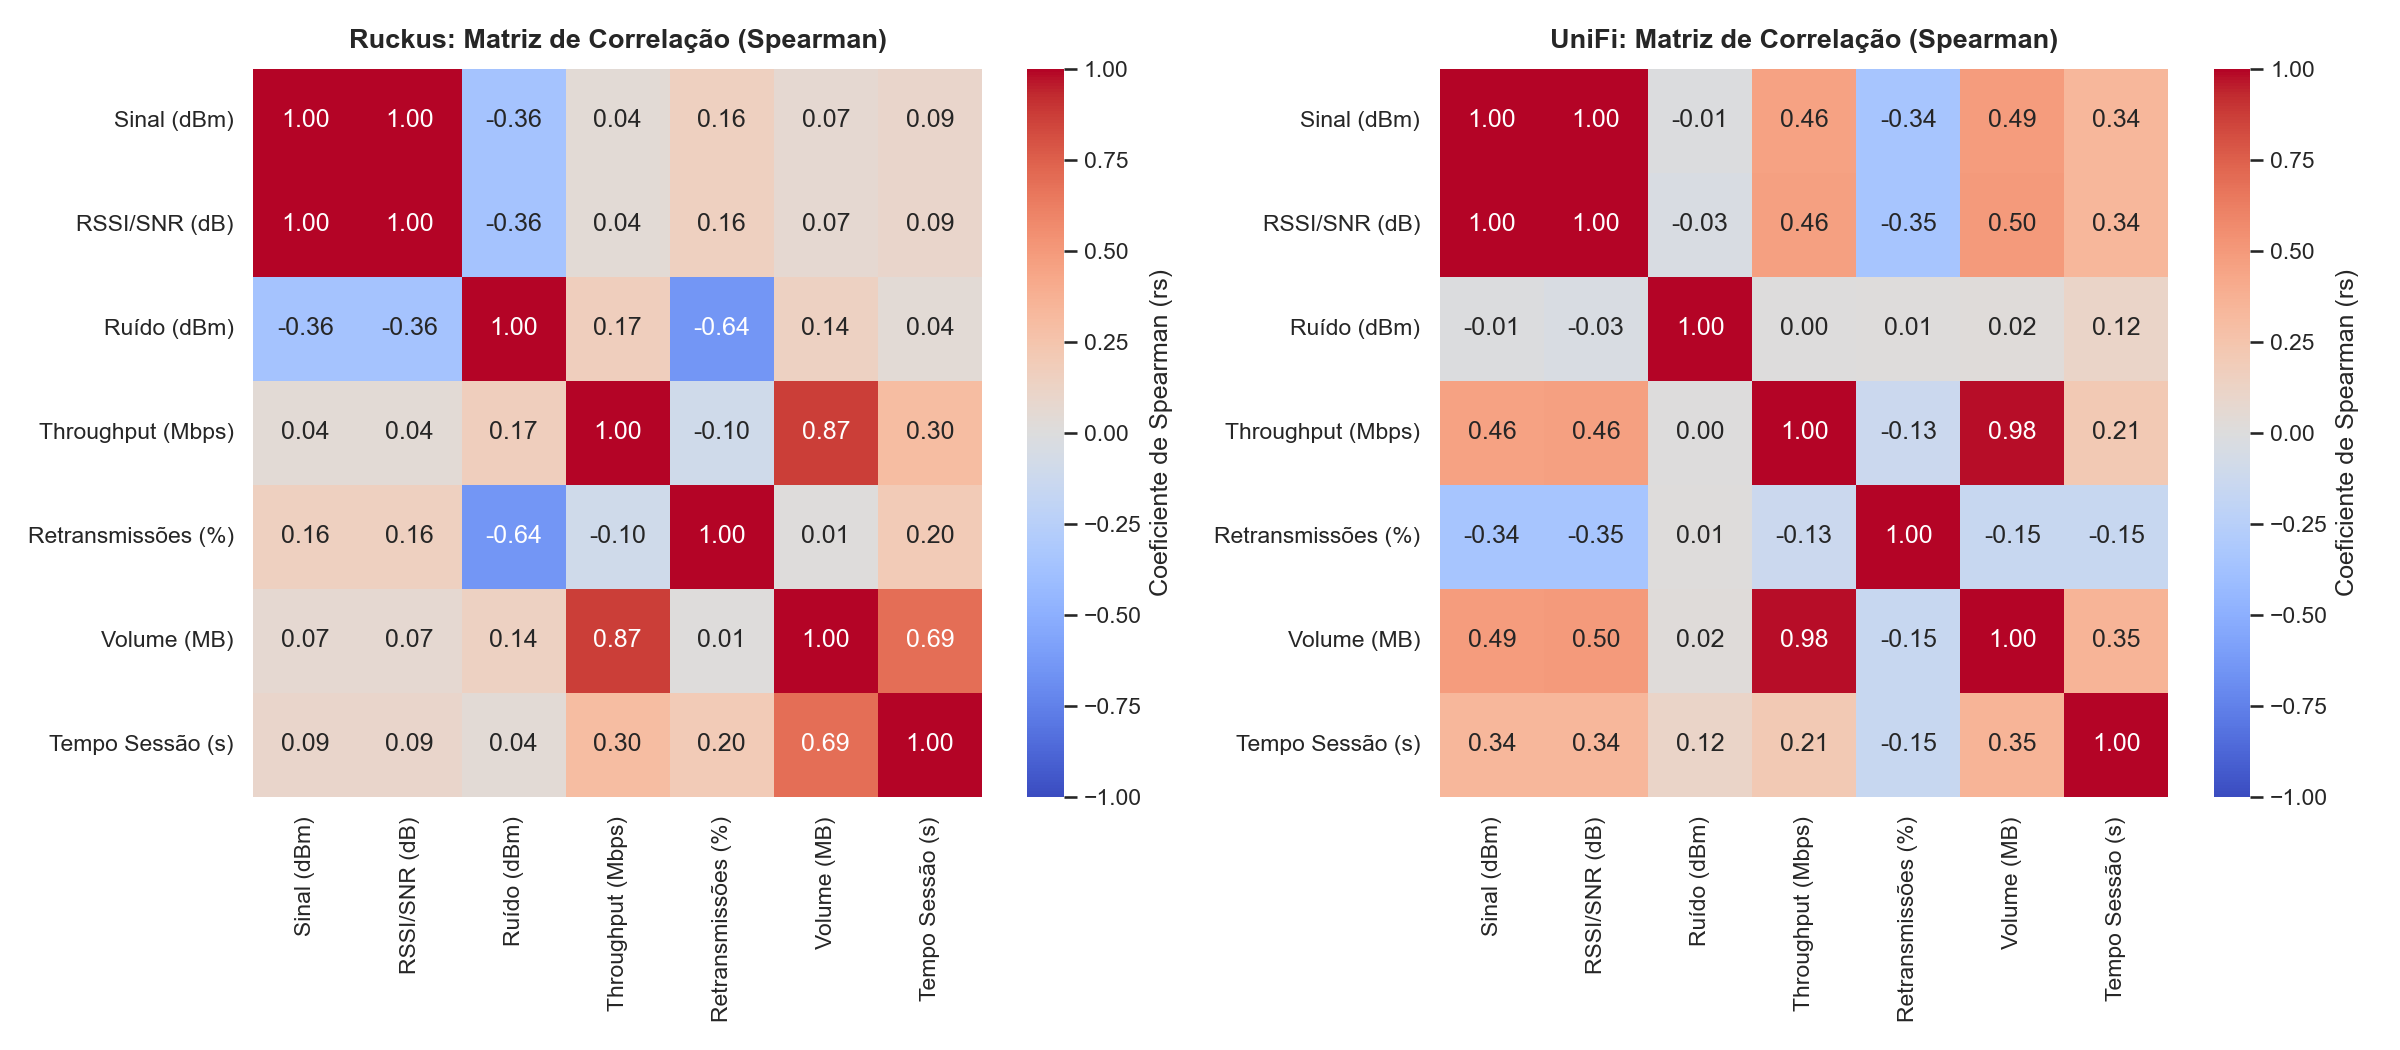
\includegraphics[width=\textwidth]{img/matriz_correlacao_heatmap.png}}
                    \caption{Matriz de Correlação de Spearman \quad \hyperlink{zoom_correlacoes}{\beamergotobutton{Ampliar}}}
                    \label{fig:correlacao_heatmap}
                \end{figure}
            \end{column}
        \end{columns}
    \end{frame}
    \note{
        \scriptsize
        \textbf{[Tempo: ~1,5 min | Roteiro de Fala - Correlações de Spearman]}\\[2pt]
        $\bullet$ \textbf{Por que Spearman em vez de Pearson?} Como comprovado pelo teste de Shapiro-Wilk, as métricas de rede não seguem distribuição normal. Spearman avalia associações monotônicas sem o viés de linearidade.\\[2pt]
        $\bullet$ \textbf{Achado Contraintuitivo (Sinal x Throughput = 0,04):} Este é um ponto de ouro para destacar à banca! O senso comum diz: ``se estou colado no AP com 5 barras de sinal (-50 dBm), minha internet vai voar''. Os dados empíricos provam que a correlação é quase NULA ($r_s = 0,04$). Por quê? No CSMA/CA, você divide o tempo aéreo com outros 20 ou 30 aparelhos; além disso, a maioria está ociosa, demandando dados sob demanda da aplicação.\\[2pt]
        $\bullet$ \textbf{Clientes x Carga Agregada ($r_s = 0,79$ RK e $0,53$ UF):} Confirmação de que o tráfego agregado no AP responde diretamente à densidade de estações ativas.\\[2pt]
        $\bullet$ \textbf{Clientes x Retransmissões ($r_s = 0,35$ e $0,21$):} A física do protocolo DCF do IEEE 802.11: quanto mais clientes concorrem pelo canal, maior a probabilidade de colisão simultânea de quadros e retransmissões.
    }

    \begin{frame}[label=slide_testes]{Resultados}{Inferência Estatística e Desbalanceamento (Jain)}
        \begin{columns}
            \begin{column}{0.50\textwidth}
                \scriptsize
                \begin{itemize}
                    \item \textbf{Não-Normalidade (Shapiro-Wilk)}: Rejeição categórica da normalidade ($p < 0,001$) em todas as métricas, justificando testes não-paramétricos.
                    \item \textbf{Diferenças Físicas (Mann-Whitney U)}: Disparidades comprovadas ($p < 0,001$) em Sinal Físico, Retransmissões e Throughput.
                    \item \textbf{Tamanho de Efeito ($r$ de Rosenthal)}:
                        \begin{itemize}
                            \scriptsize
                            \item Retransmissões Geral: $r = 0,3613$ (Médio).
                            \item Retransmissões RK (2,4G vs 5G): $r = 0,5221$ (\textbf{Grande}).
                        \end{itemize}
                    \item \textbf{Índice de Jain ($p < 0,001, r = 0,4484$)}:
                        \begin{itemize}
                            \scriptsize
                            \item Mediana: \textbf{0,26} (RK) e \textbf{0,14} (UF); Q3 de apenas \textbf{0,44}.
                            \item \textbf{Severo Desbalanceamento}: Na escala de $1/40 = 0,025$ a $1,0$ (equidade ideal), valores abaixo de 0,50 comprovam que a demanda é altamente concentrada em poucos APs.
                        \end{itemize}
                \end{itemize}
            \end{column}
            \begin{column}{0.50\textwidth}
                \begin{figure}
                    \centering
                    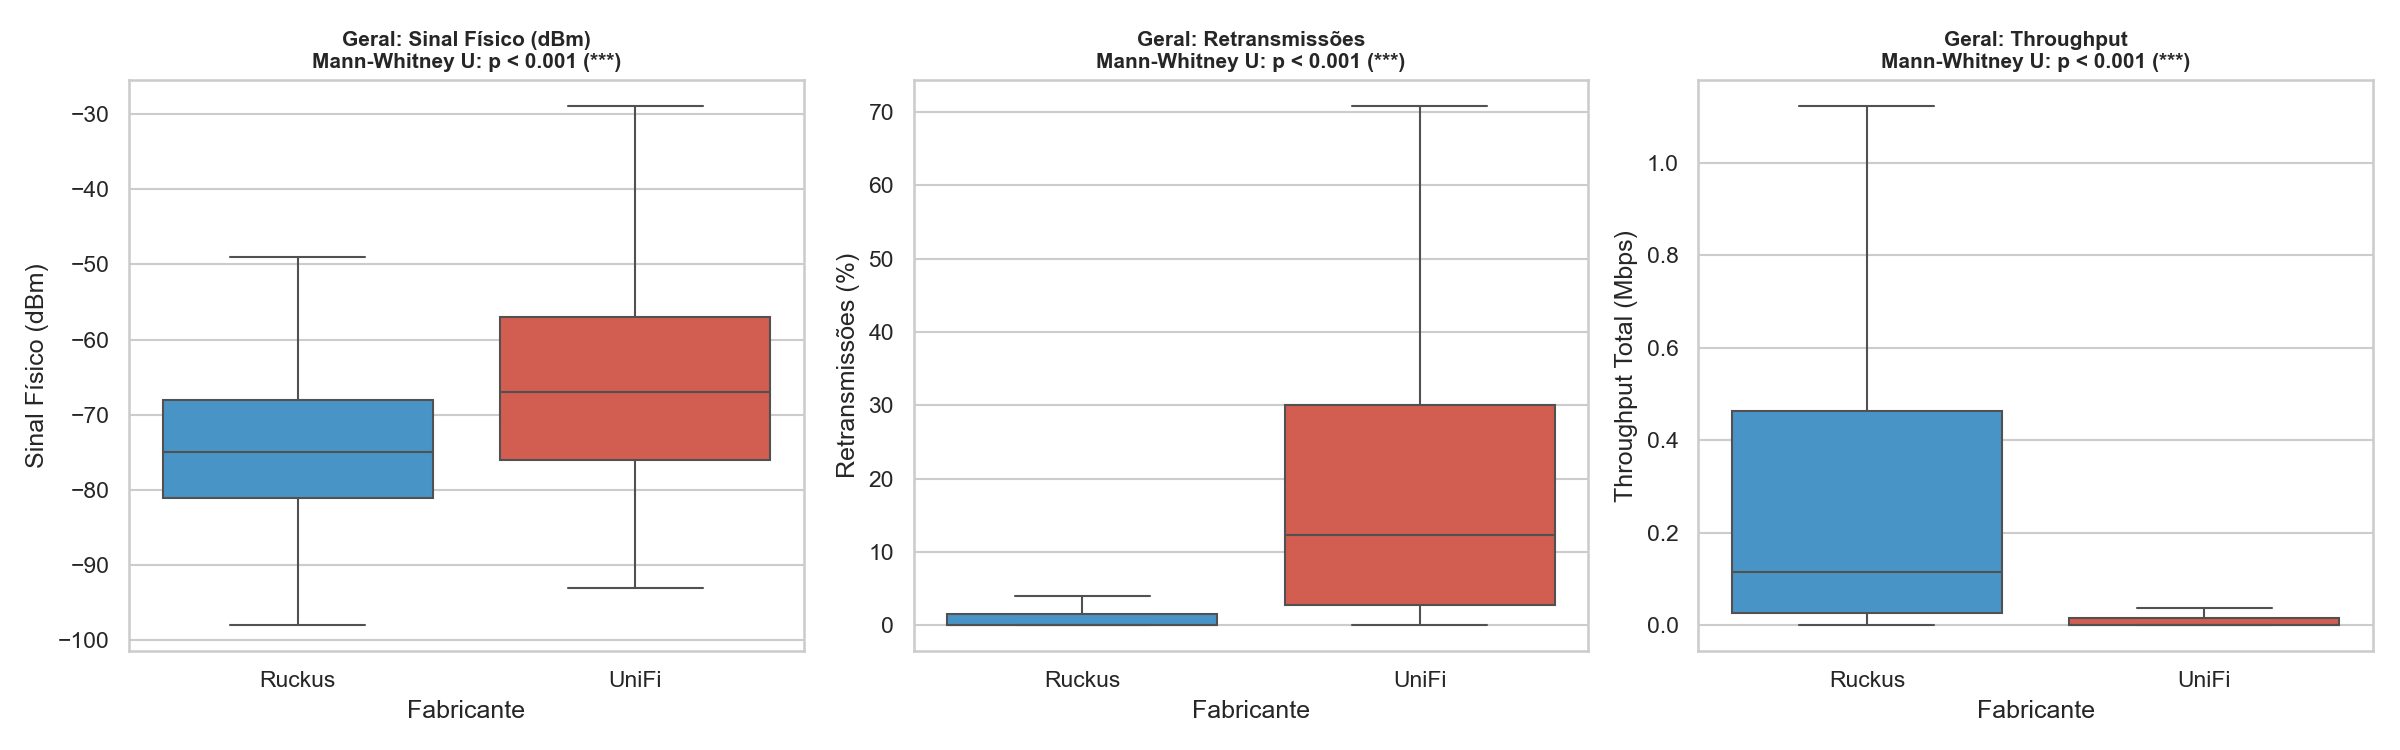
\includegraphics[width=\textwidth]{img/03_fabricantes_geral_comparacao.png}
                    \caption{Comparação Geral de Fabricantes ($p < 0,001$)}
                    \label{fig:testes_comparacao_slide}
                \end{figure}
                \vspace{-0.2cm}
                \centering
                \hyperlink{zoom_jain}{\beamergotobutton{Ampliar Equidade (Jain)}}
            \end{column}
        \end{columns}
    \end{frame}
    \note{
        \scriptsize
        \textbf{[Tempo: ~2 min | Roteiro de Fala - Inferência Estatística e Jain]}\\[2pt]
        $\bullet$ \textbf{O que significa $p < 0,001$?} O $p$-valor mede a probabilidade de o resultado ter ocorrido por pura coincidência. Dizer $p < 0,001$ significa que a chance de erro é menor que 0,1\% --- temos \textbf{mais de 99,9\% de certeza matemática} de que as diferenças entre Ruckus e UniFi são reais.\\[2pt]
        $\bullet$ \textbf{1. Shapiro-Wilk ($p < 0,001$):} Rejeita a distribuição normal. O tráfego de rede é assimétrico por natureza (poucos clientes baixam muito, a maioria é ociosa). Isso prova metodologicamente que usar o teste $t$ de Student seria um erro grave.\\[2pt]
        $\bullet$ \textbf{2. Tamanho de Efeito ($r$ de Rosenthal):} O $p$-valor diz que ``há diferença'', mas o $r$ mede a \textbf{relevância prática}: o ganho de 5 GHz vs 2,4 GHz na Ruckus teve efeito grande ($r = 0,5221$), embasando a recomendação de Band Steering.\\[2pt]
        $\bullet$ \textbf{3. O Índice de Equidade de Jain (Ponto Crucial):} O índice varia de $1/N = 1/40 = 0,025$ (pior caso teórico, onde 1 rádio concentra tudo e 39 ficam vazios) até $1,0$ (balanceamento perfeito). Nossos dados mostram mediana de \textbf{0,26} na Ruckus e \textbf{0,14} na UniFi, com terceiro quartil de apenas 0,44. \textbf{Atenção para a banca: 0,26 a 0,44 NÃO é balanceado!} Em engenharia de redes, qualquer valor abaixo de 0,50 é prova matemática de um \textbf{severo desbalanceamento de carga}. Poucos APs concentram turmas inteiras (50 a 64 alunos), gerando o Gargalo G2, enquanto dezenas de outros APs ficam ociosos. Se a banca quiser ver os detalhes, clique no botão \textit{Ampliar Equidade (Jain)}!
    }

    \begin{frame}{Resultados}{Classificação Determinística de Gargalos}
        \begin{columns}
            \begin{column}{0.48\textwidth}
                \scriptsize
                \begin{itemize}
                    \item \textbf{G1: Baixa Qualidade de Enlace} (43,1\% RK / 26,3\% UF): Atenuação física por paredes de alvenaria.
                    \item \textbf{G2: Congestionamento do Meio} (44,5\% RK / 2,6\% UF): Alta concentração em salas atendidas pela Ruckus.
                    \item \textbf{G3: Interferência / SNR Ruim} (0,0\% RK / 1,1\% UF): Ruído em canal 2,4 GHz isolado na UniFi.
                    \item \textbf{G4: Instabilidade de Roaming} (58,9\% RK / 24,3\% UF): Prevalente por circulação entre blocos e \textit{sticky clients}.
                    \item \textbf{G5: Gargalo Cabeado (Fast Ethernet)} ($< 0,01\%$ RK / 0,0\% UF): Apenas 33 amostras em 446k $\rightarrow$ \textbf{o cabeamento não é o gargalo}.
                \end{itemize}
            \end{column}
            \begin{column}{0.52\textwidth}
                \begin{figure}
                    \centering
                    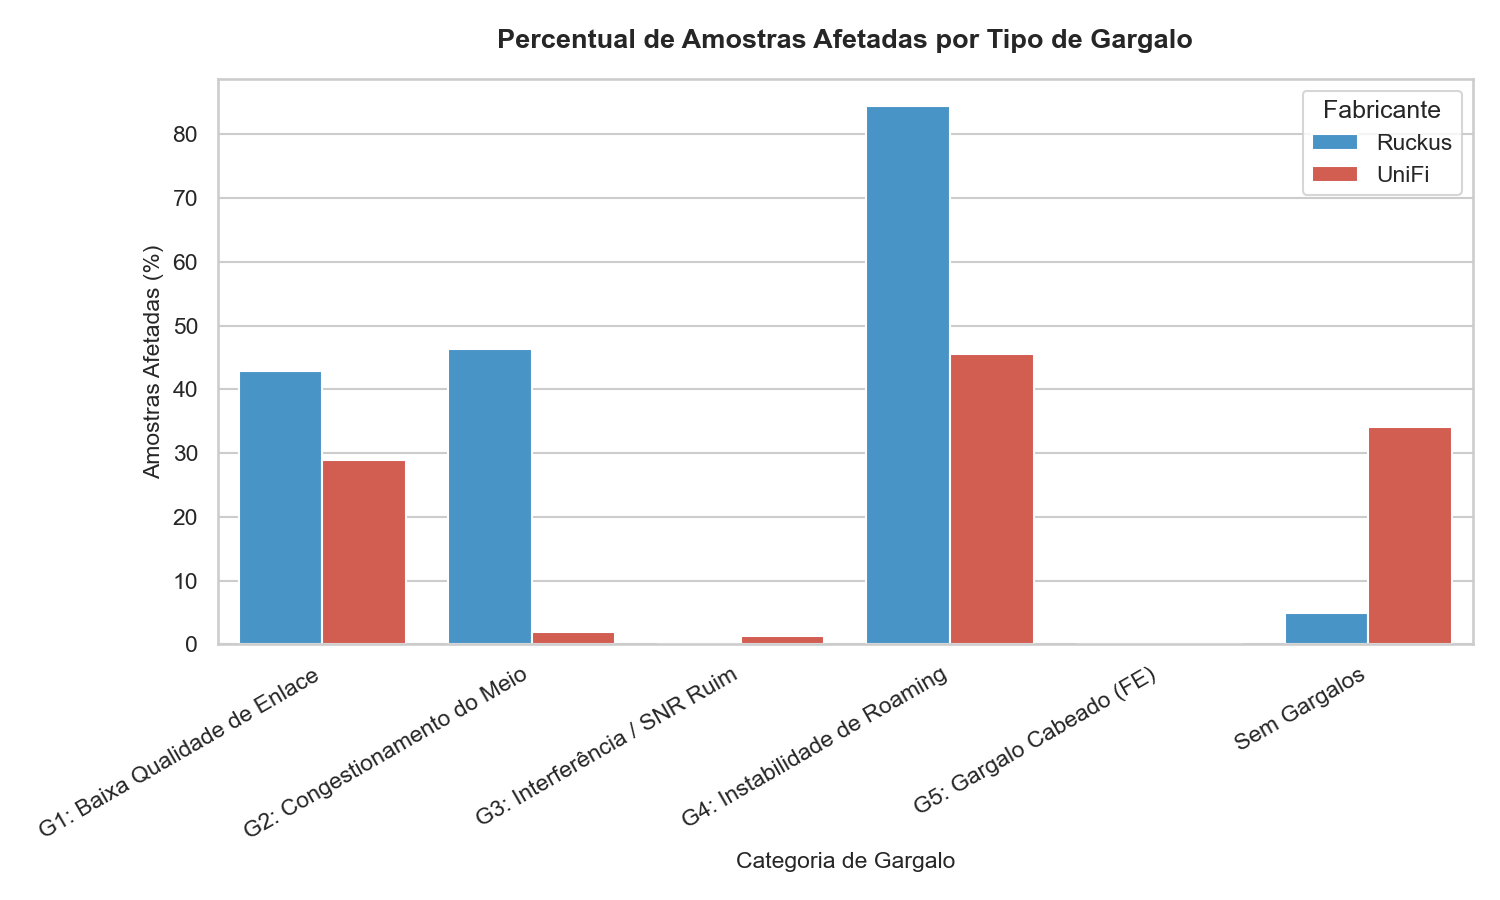
\includegraphics[width=\textwidth]{img/distribuicao_gargalos.png}
                    \caption{Prevalência Relativa dos Gargalos Físicos e Lógicos}
                    \label{fig:distribuicao_gargalos_slides}
                \end{figure}
            \end{column}
        \end{columns}
    \end{frame}
    \note{
        [~1,5 min] Distribuição ordenada dos gargalos G1 a G5 no campus: \\
        G1 (Baixa Qualidade de Enlace): 43,1\% RK e 26,3\% UF devido a atenuação física por paredes. \\
        G2 (Congestionamento do Meio): 44,5\% no Ruckus (salas cheias de aula) vs 2,6\% na UniFi. \\
        G3 (Interferência / SNR Ruim): residual (1,1\% na UniFi e 0\% no Ruckus). \\
        G4 (Instabilidade de Roaming): mais frequente (58,9\% RK / 24,3\% UF) por mobilidade e sticky clients. \\
        G5 (Gargalo Cabeado FE): apenas 33 amostras em quase meio milhão (< 0,01\%). O cabeamento definitivamente não é o gargalo da UFOP.
    }

    \begin{frame}{Resultados}{Validação Não-Supervisionada dos APs (K-Means)}
        \begin{columns}
            \begin{column}{0.48\textwidth}
                \begin{block}{Propósito da Modelagem}
                    Auditar e validar os diagnósticos \textbf{sem pré-julgamentos ou regras manuais}, agrupando os 40 APs por semelhança de comportamento físico.
                \end{block}
                \scriptsize
                \textbf{Vetor de Features por AP ($X_j$)}:
                $$X_j = \{ C_j, T_j, S_j, R_j \}$$
                \begin{itemize}
                    \item $C_j$: Clientes médios | $T_j$: Throughput (Mbps)
                    \item $S_j$: Sinal físico (dBm) | $R_j$: Retransmissão (\%)
                \end{itemize}
                Padronização $z$-score (\textit{StandardScaler}) para equalizar grandezas de RF e contagem.
            \end{column}
            \begin{column}{0.52\textwidth}
                \begin{figure}
                    \centering
                    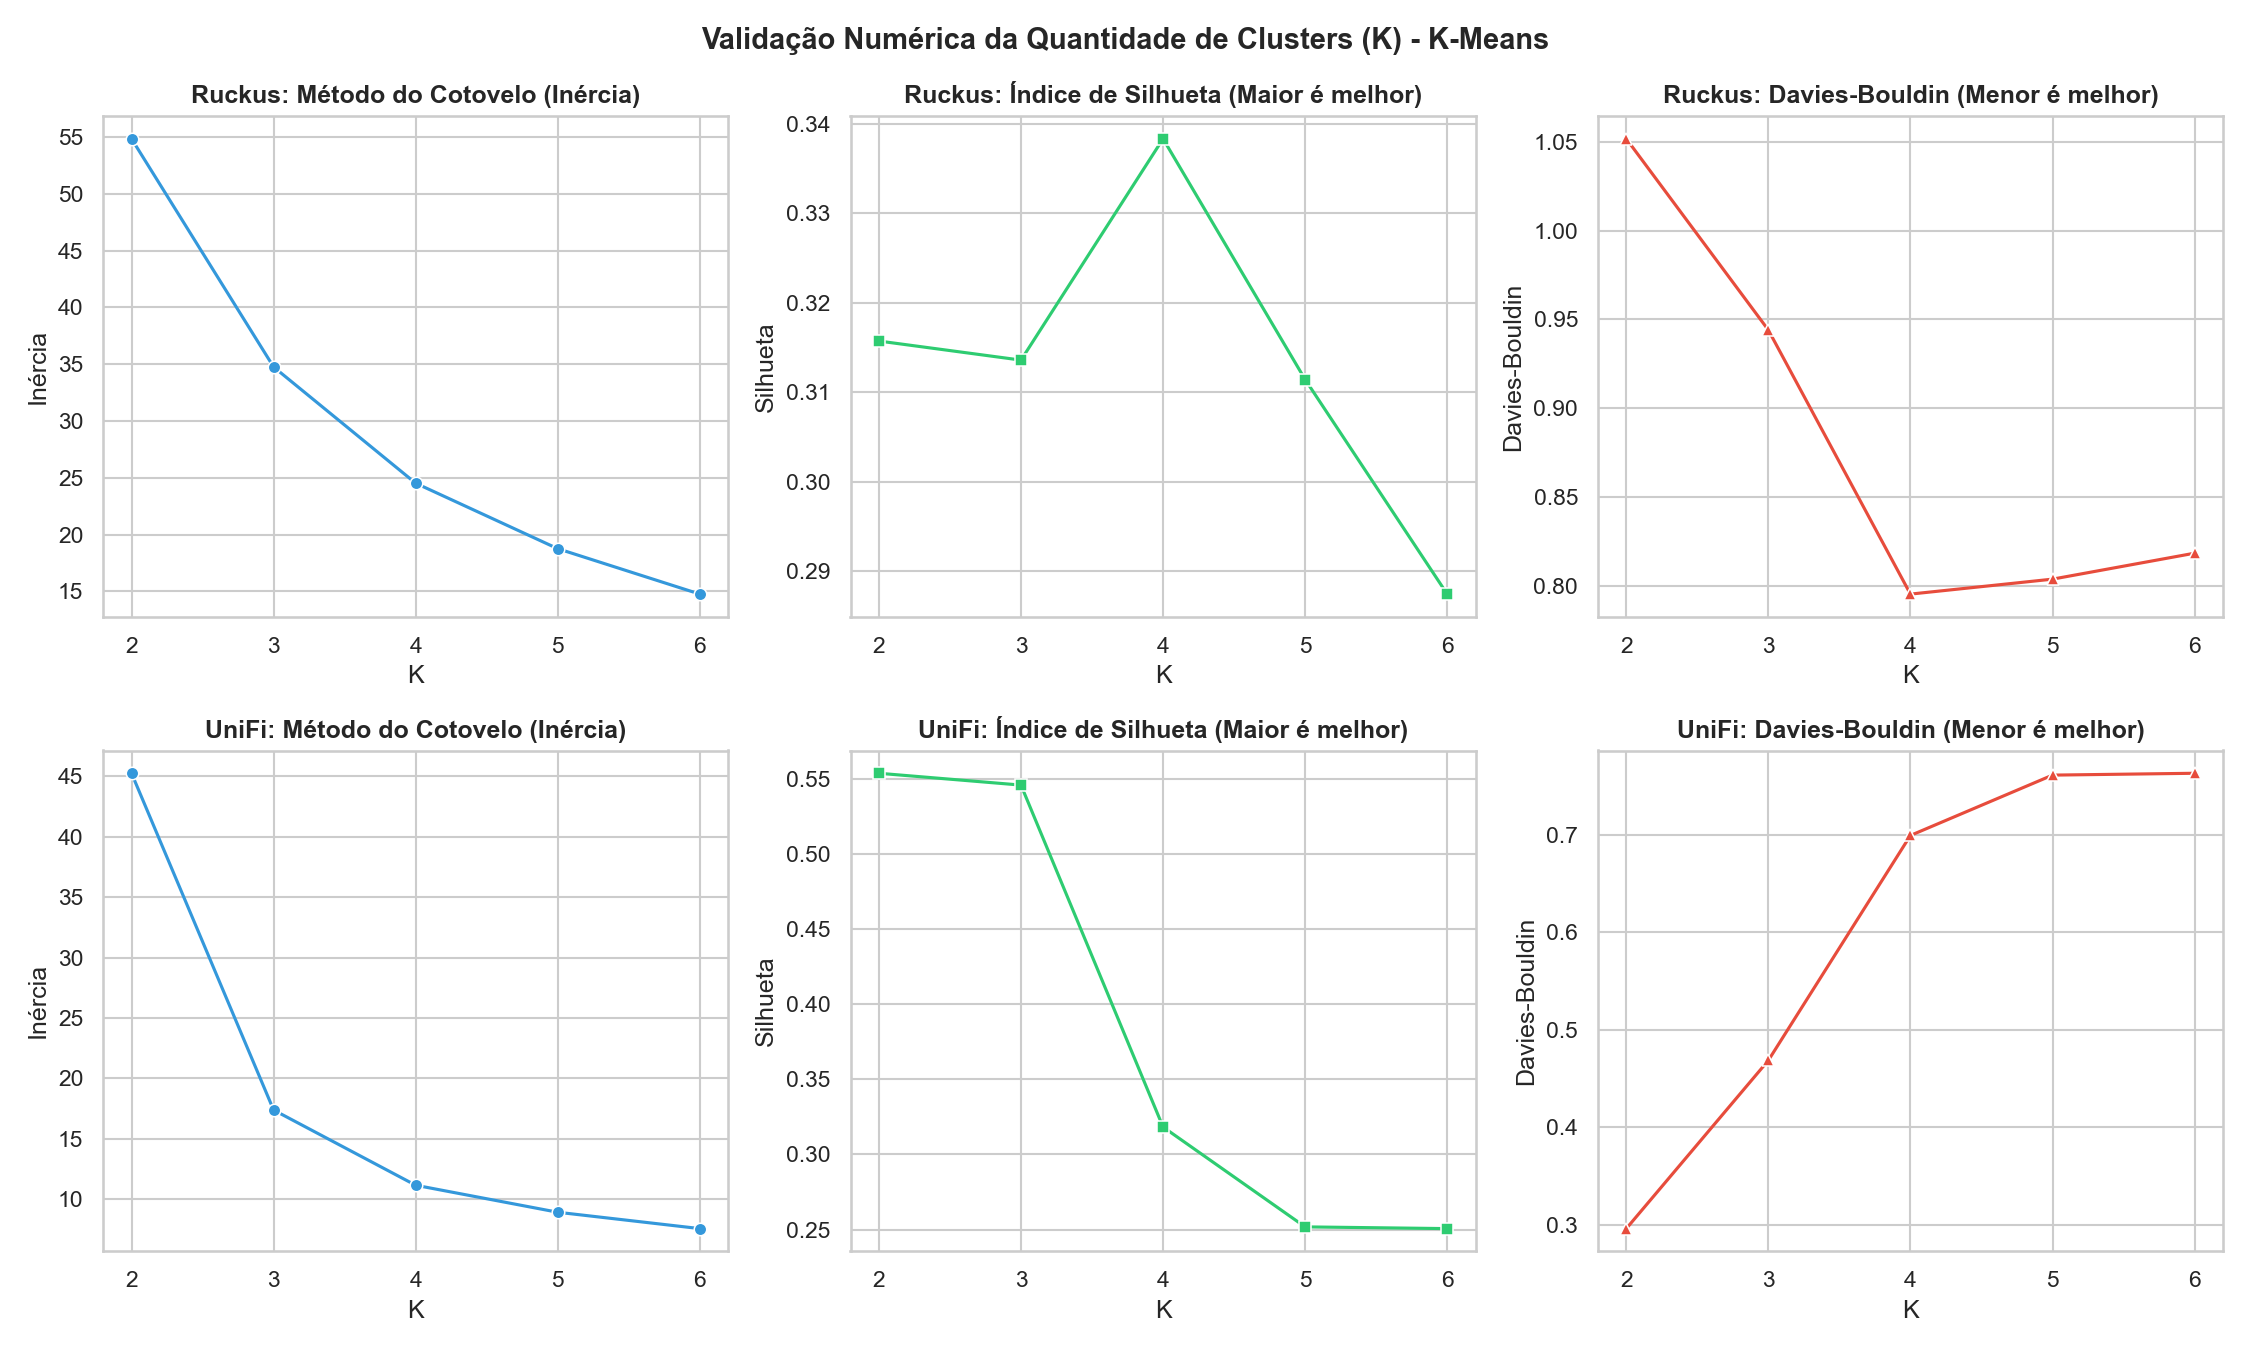
\includegraphics[width=\textwidth]{img/validador_kmeans_metricas.png}
                    \caption{Convergência Matemática para $K=4$}
                    \label{fig:validador_kmeans_slides}
                \end{figure}
                \scriptsize
                Convergência simultânea: Cotovelo de inércia estável, Silhueta máxima ($0,3383$) e Davies-Bouldin mínimo ($0,7953$).
            \end{column}
        \end{columns}
    \end{frame}
    \note{
        \scriptsize
        \textbf{[Tempo: ~1,5 min | Validação K-Means]}\\[2pt]
        $\bullet$ \textbf{Por que K-Means aqui?} Acabamos de ver os gargalos determinísticos G1 a G5. A banca poderia questionar: essas regras não foram subjetivas? Para responder a isso, aplicamos o K-Means para auditar os 40 APs sem viés humano.\\[2pt]
        $\bullet$ \textbf{Vetor de Features ($X_j$):} Cada AP é representado por 4 métricas físicas ($C_j$ clientes médios, $T_j$ vazão, $S_j$ sinal e $R_j$ perdas), padronizadas em escore-$z$ para equalizar grandezas de dBm e Mbps.\\[2pt]
        $\bullet$ \textbf{Convergência Matemática em $K=4$:} Mostre o gráfico à direita com as 3 curvas: Cotovelo de inércia estável, pico global da Silhueta ($0,3383$) e mínimo de Davies-Bouldin ($0,7953$). Isso prova que 4 clusters é a partição natural da rede. Vejamos agora esses 4 perfis em cada fabricante!
    }

    \begin{frame}{Resultados}{Agrupamento K-Means -- Perfis Ruckus}
        \begin{columns}
            \begin{column}{0.5\textwidth}
                \scriptsize
                \begin{itemize}
                    \item \textbf{Grupo A (Muito Carregado)}: Alta densidade (21,7 clientes) e tráfego elevado (13,25 Mbps), mantendo baixa retransmissão (\textbf{3,90\%}) por direcionamento adaptativo de feixe (BeamFlex).
                    \item \textbf{Grupo B (Pouco Utilizado)}: 6,4 clientes e 2,82 Mbps em operação saudável (-72,3 dBm).
                    \item \textbf{Grupo C (Carga Moderada)}: 14,9 clientes e 6,43 Mbps (padrão nominal do campus).
                    \item \textbf{Grupo D (Sinal Degradado)}: Rádios com IS atenuada (-75,3 dBm) e retransmissão de \textbf{8,96\%}. Valida o Gargalo G1.
                \end{itemize}
            \end{column}
            \begin{column}{0.5\textwidth}
                \begin{figure}
                    \centering
                    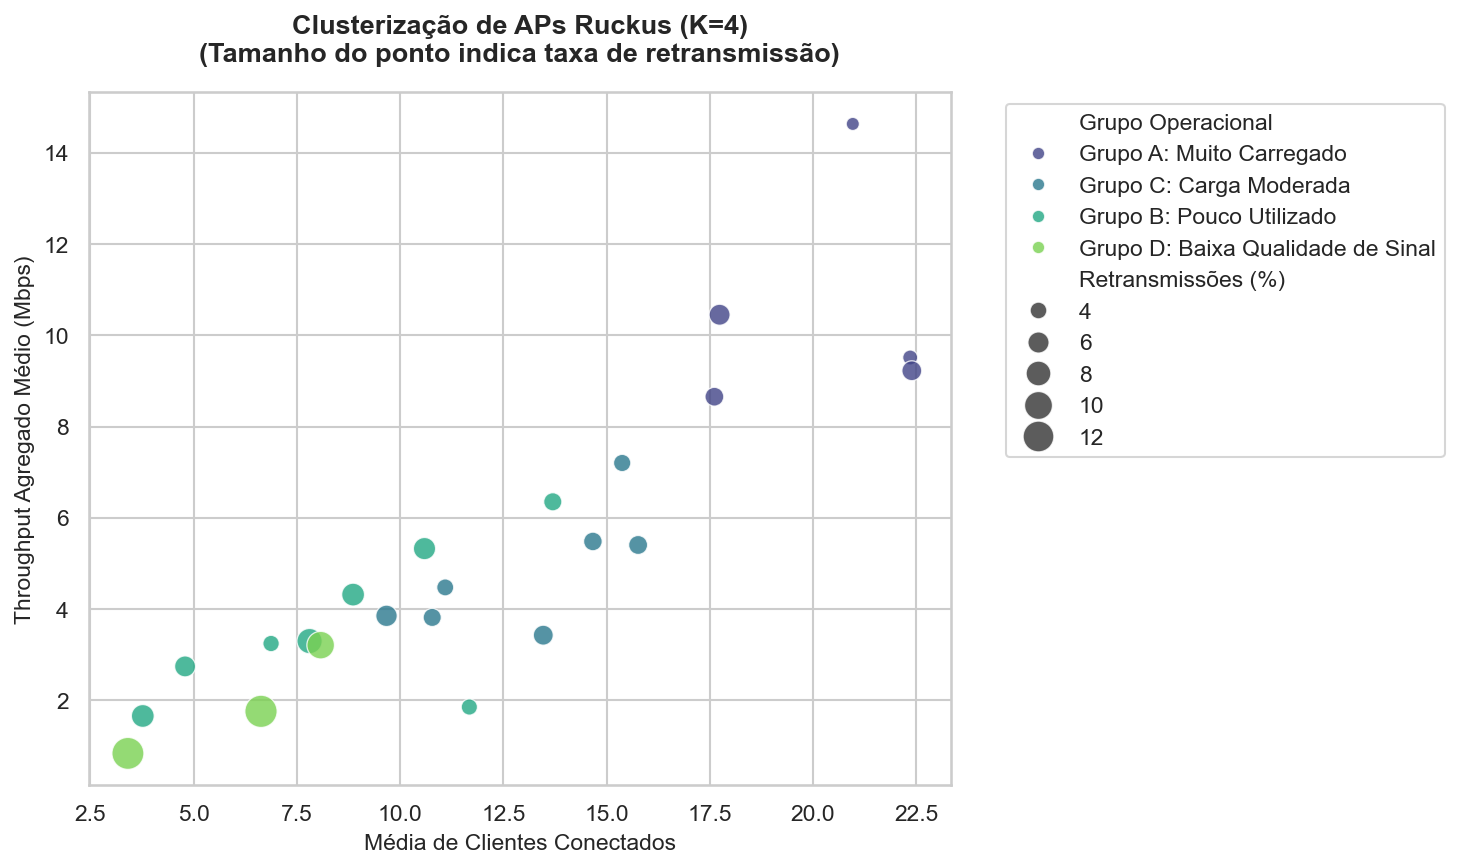
\includegraphics[width=0.88\textwidth]{img/cluster_ruckus.png}
                    \caption{Perfis de APs Ruckus (Centróides)}
                    \label{fig:cluster_ruckus_slides}
                \end{figure}
            \end{column}
        \end{columns}
    \end{frame}
    \note{
        \footnotesize
        \textbf{[Tempo: ~1,5 min | Roteiro de Fala - K-Means Ruckus]}\\[2pt]
        $\bullet$ \textbf{Objetivo do Clustering:} Validar sem supervisão humana os perfis de operação dos 23 APs Ruckus, confirmando as heurísticas.\\[2pt]
        $\bullet$ \textbf{Grupo A (Muito Carregado - O Destaque da Ruckus):} 21,7 clientes médios e 13,25 Mbps de tráfego agregado. Ponto crucial para falar à banca: mesmo sob carga pesada, a taxa de perda foi de apenas \textbf{3,90\%}! Explique que as antenas inteligentes \textit{BeamFlex} direcionam feixes ao cliente ativo e suprimem interferências, absorvendo o Gargalo G2 com excelência.\\[2pt]
        $\bullet$ \textbf{Grupo C (Carga Moderada):} 14,9 clientes e 6,43 Mbps. Representa o padrão nominal e saudável das salas de aula do ICEA.\\[2pt]
        $\bullet$ \textbf{Grupo B (Pouco Utilizado):} 6,4 clientes e 2,82 Mbps em operação leve.\\[2pt]
        $\bullet$ \textbf{Grupo D (Sinal Degradado):} Sinal atenuado em -75,3 dBm e perda sobe para \textbf{8,96\%}. Valida o Gargalo G1 (atenuação por paredes espessas).
    }

    \begin{frame}{Resultados}{Agrupamento K-Means -- Perfis UniFi}
        \begin{columns}
            \begin{column}{0.5\textwidth}
                \scriptsize
                \begin{itemize}
                    \item \textbf{Grupo A (Muito Carregado)}: Com apenas 6,35 clientes, retransmissões chegam a \textbf{25,13\%}, indicando contenção no canal 2,4 GHz (Gargalo G2).
                    \item \textbf{Grupo B (Pouco Utilizado)}: 1,67 clientes e tráfego de 0,17 Mbps, com 23,24\% de retransmissão induzida por ruído de fundo.
                    \item \textbf{Grupo C (Anomalia de RF -- PICO-H-100)}: Sinal excelente (\textbf{-46,1 dBm}), mas perda crítica de \textbf{35,49\%}. Anomalia física localizada que demanda \textit{site survey} ativo.
                    \item \textbf{Grupo D (Estável)}: Menor retransmissão da UniFi (15,67\%) sob 2,41 clientes.
                \end{itemize}
            \end{column}
            \begin{column}{0.5\textwidth}
                \begin{figure}
                    \centering
                    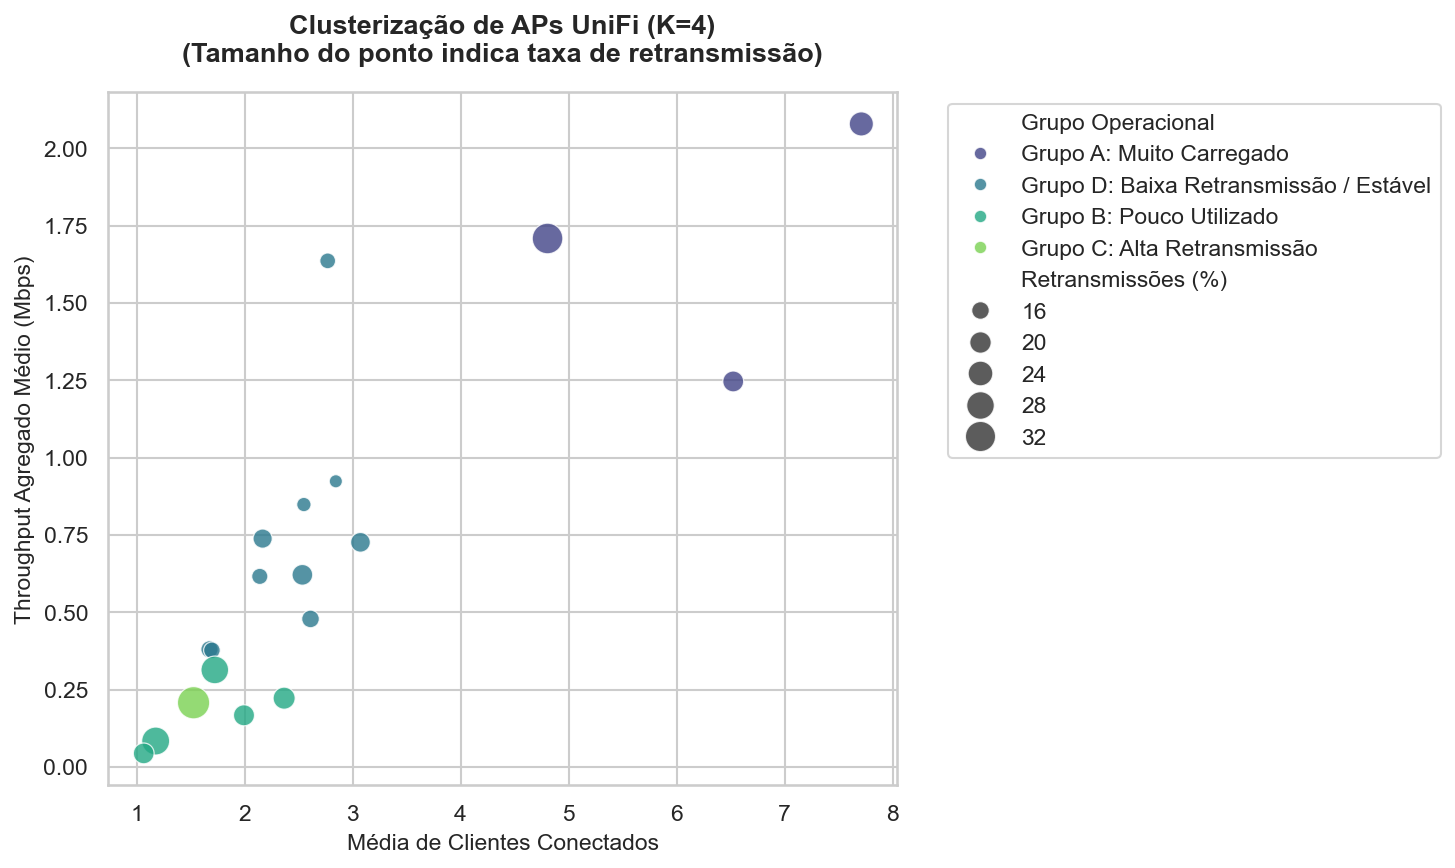
\includegraphics[width=0.88\textwidth]{img/cluster_unifi.png}
                    \caption{Perfis de APs UniFi (Centróides)}
                    \label{fig:cluster_unifi_slides}
                \end{figure}
            \end{column}
        \end{columns}
    \end{frame}
    \note{
        \footnotesize
        \textbf{[Tempo: ~2 min | Roteiro de Fala - K-Means UniFi]}\\[2pt]
        $\bullet$ \textbf{Contraste com a Ruckus:} A UniFi opera exclusivamente em 2,4 GHz em canal de 20 MHz sem conformação dinâmica de feixes, sofrendo muito mais com contenção.\\[2pt]
        $\bullet$ \textbf{Grupo A (Muito Carregado):} Bastam \textbf{6,35 clientes} para que as retransmissões atinjam \textbf{25,13\%} por colisão CSMA/CA no canal 2,4 GHz.\\[2pt]
        $\bullet$ \textbf{Grupo C (Anomalia de RF no AP PICO-H-100):} Os clientes apresentam sinal excelente (\textbf{-46,1 dBm}, estações próximas ao rádio), mas uma taxa de perda alarmante de \textbf{35,49\% de quadros}!\\[2pt]
        $\bullet$ \textbf{Rigor Metodológico (Aviso para a Banca):} Seria precipitado cravar que isso é mero desbalanço de potência AP-cliente sem medições laboratoriais de bancada da transmissão dos aparelhos móveis. A conduta científica e segura é diagnosticar o Grupo C como uma \textbf{anomalia severa de RF} e recomendar uma investigação em campo via \textit{site survey} ativo no setor do AP \texttt{PICO-H-100} para inspecionar fontes pontuais de interferência destrutiva, reflexões ou nós escondidos.\\[2pt]
        $\bullet$ \textbf{Grupos B e D:} Com 1,67 e 2,41 clientes, perdem de 15\% a 23\% por ruído de fundo permanente da faixa de 2,4 GHz.
    }

    \section{Recomendações e Ações}
    \begin{frame}{Recomendações e Ações de Verificação}
        Com base no diagnóstico empírico dos gargalos e clusters, propomos ações de engenharia de redes viáveis e de baixo custo:
        
        \begin{block}{1. Cobertura Física e Atenuação (Gargalo G1 e Grupo D Ruckus)}
            Realizar \textit{site survey} nos setores com sinal atenuado (ex.: APs RK-3440 e RK-dcd0) antes de reposicionar APs para contornar divisórias espessas de alvenaria.
        \end{block}
        
        \begin{block}{2. Gerência de Tráfego e Contenção (Gargalos G2 e G3)}
            Ativação de \textbf{Band Steering} nas controladoras para direcionar clientes compatíveis para a faixa de 5 GHz, aliviando o espectro saturado de 2,4 GHz.
        \end{block}
        
        \begin{block}{3. Auditoria Espectral via Site Survey Ativo (Grupo C UniFi)}
            Executar medição ativa de campo no setor do AP \texttt{PICO-H-100} para rastrear fontes de ruído pontual, reflexões severas ou assimetrias de enlace antes de intervir nas configurações de rádio.
        \end{block}
    \end{frame}
    \note{
        \scriptsize
        \textbf{[Tempo: ~1,5 min | Roteiro de Fala - Recomendações e Ações]}\\[2pt]
        $\bullet$ \textbf{1. Site survey e reposicionamento (G1):} Em vez de comprar novos equipamentos, mapear as zonas de sombra causadas pela alvenaria do campus e planejar o reposicionamento físico dos APs com sinal degradado.\\[2pt]
        $\bullet$ \textbf{2. Band Steering (G2/G3):} Ação imediata e de \textbf{custo zero} via software na controladora para empurrar dispositivos de 2,4 GHz para 5 GHz, aliviando o espectro saturado (apoiada pelo efeito grande $r = 0,5221$ comprovado no Mann-Whitney).\\[2pt]
        $\bullet$ \textbf{3. Site Survey Ativo no AP PICO-H-100 (Grupo C):} Como detectamos que esse rádio opera com sinal excelente e 35\% de retransmissões, a ação prática de engenharia é levar um dispositivo de teste ao local físico do AP para auditar o espectro de RF e descobrir o que está destruindo os quadros antes de aplicar qualquer ajuste.
    }

    \section{Conclusões}
    \begin{frame}{Conclusões}
        \begin{itemize}
            \item Caracterização de um dataset de produção com \textbf{498.034 registros de telemetria reais} no campus (20 dias úteis divididos em duas fases letivas), fornecendo diagnóstico empírico inédito.
            \item A insatisfação dos usuários decorre de \textbf{severo desbalanceamento de carga} (Índice de Jain mediano de 0,26 RK / 0,14 UF), contenção CSMA/CA e anomalias de RF, e \textbf{não} do link de internet ou infraestrutura cabeada (Gargalo G5 $<0,01\%$).
            \item A modelagem K-Means validou sem supervisão os perfis operacionais da infraestrutura, identificando com sucesso células saudáveis sob carga e isolando a anomalia severa de RF do AP \texttt{PICO-H-100}.
            \item As intervenções recomendadas (\textit{site survey} ativo e \textit{Band Steering}) são de \textbf{baixo custo e alto impacto}, garantindo melhorias imediatas na Qualidade de Experiência (QoE) da comunidade acadêmica.
        \end{itemize}
        
        \begin{block}{Trabalhos Futuros}
            Monitoramento de dispositivos IoT e expansão do pipeline analítico com algoritmos supervisionados de aprendizado de máquina para previsão de anomalias em tempo real.
        \end{block}
    \end{frame}
    \note{
        \scriptsize
        \textbf{[Tempo: ~1 min | Roteiro de Fala - Conclusões]}\\[2pt]
        $\bullet$ \textbf{Os 4 Pilares Finais da Apresentação:}\\[2pt]
        1. \textbf{Dataset Robusto e Real:} Quase 500 mil registros em duas fases letivas distintas da UFOP.\\[2pt]
        2. \textbf{Desmistificação do Problema:} O gargalo da UFOP \textbf{não é a internet cabeada} (G5 é zero!). O problema é a disputa de tempo aéreo no CSMA/CA em APs sobrecarregados (provado matematicamente pelo Índice de Jain de 0,26).\\[2pt]
        3. \textbf{Validação K-Means:} Agrupamento não-supervisionado que confirmou a excelência do BeamFlex da Ruckus e isolou anomalias na UniFi sem viés humano.\\[2pt]
        4. \textbf{Ações de Baixo Custo:} Soluções práticas de engenharia (Band Steering e Site Survey) que a própria UFOP pode implementar sem gastar milhões em infraestrutura.\\[2pt]
        $\bullet$ \textbf{Encerramento:} Agradecer à banca, ao orientador Marlon, coorientador Plínio e passar para as perguntas com total segurança.
    }

    \nologo
    \begin{frame}{Agradecimentos}
        \centering
        \huge
        \color{azul}
        Muito obrigado! \\
        ~\\
        \large
        Agradeço à banca examinadora, ao meu orientador Marlon, coorientador Plínio e à Universidade Federal de Ouro Preto. \\
        ~\\
        \large
        Perguntas?
    \end{frame}

    \begin{frame}[allowframebreaks,allowdisplaybreaks,environment=slide]{Referências}
        \frametitle{Referências}
        \bibliography{bib/decsi-cosi-modelo-monografia} 	
	\end{frame}

    % -------------------------------------------------------------------------
    % SLIDES DE ZOOM EM ALTA DEFINIÇÃO (ACESSADOS VIA CLIQUE NAS FIGURAS OU BOTÕES)
    % -------------------------------------------------------------------------
    \appendix

    \begin{frame}[plain,noframenumbering,label=zoom_heatmap]
        \begin{center}
            \hyperlink{slide_distribuicao}{%
                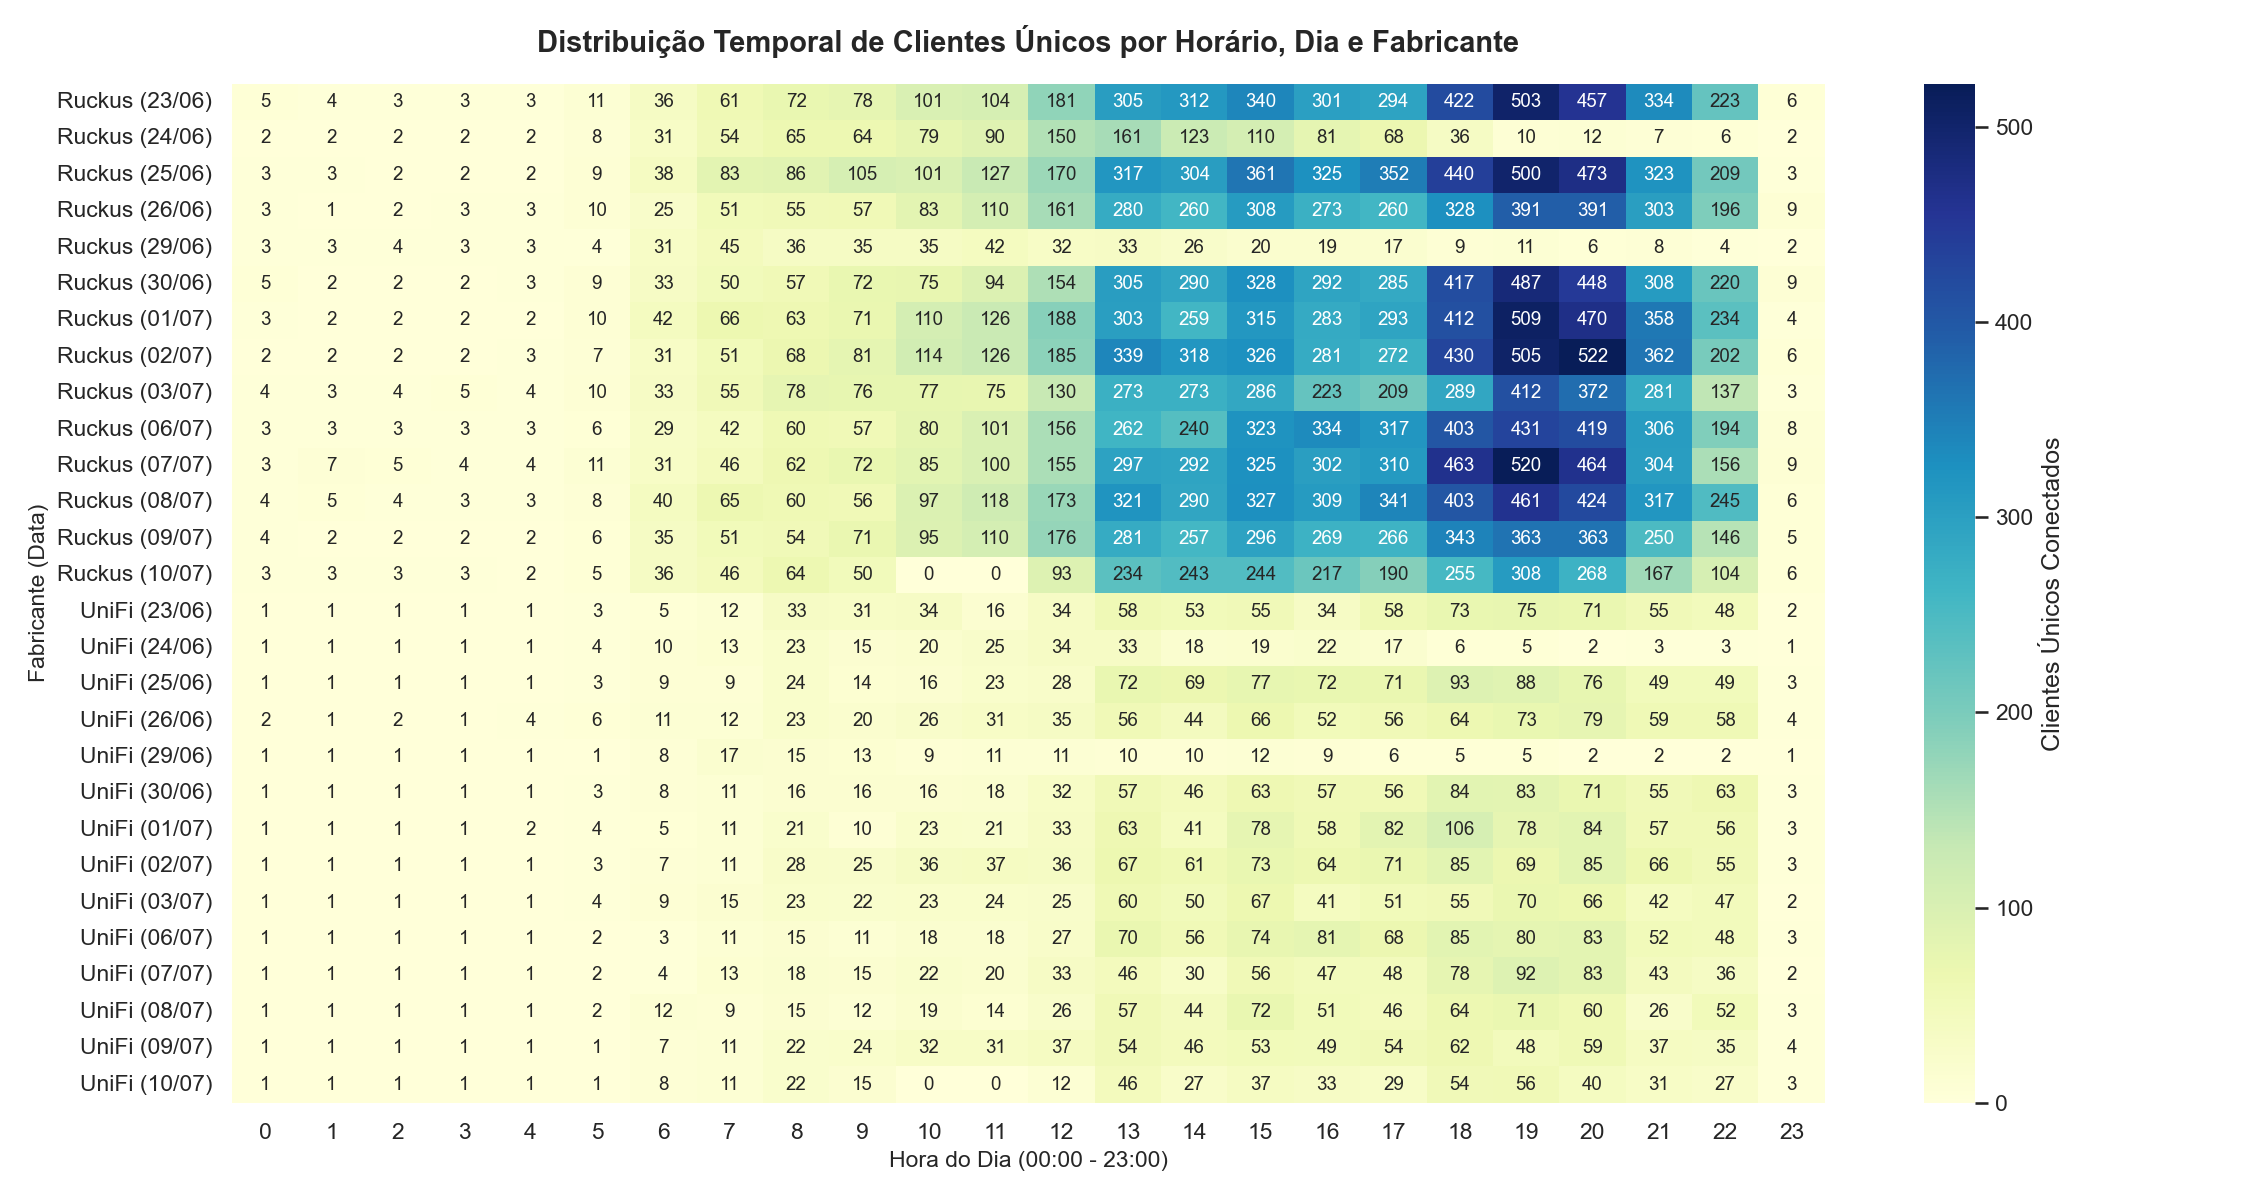
\includegraphics[width=\textwidth,height=0.88\textheight,keepaspectratio]{img/heatmap_horario_clientes.png}%
            }
        \end{center}
        \vspace{-0.2cm}
        \centering
        \hyperlink{slide_distribuicao}{\beamerreturnbutton{Voltar}}
    \end{frame}

    \begin{frame}[plain,noframenumbering,label=zoom_correlacoes]
        \begin{center}
            \hyperlink{slide_correlacoes}{%
                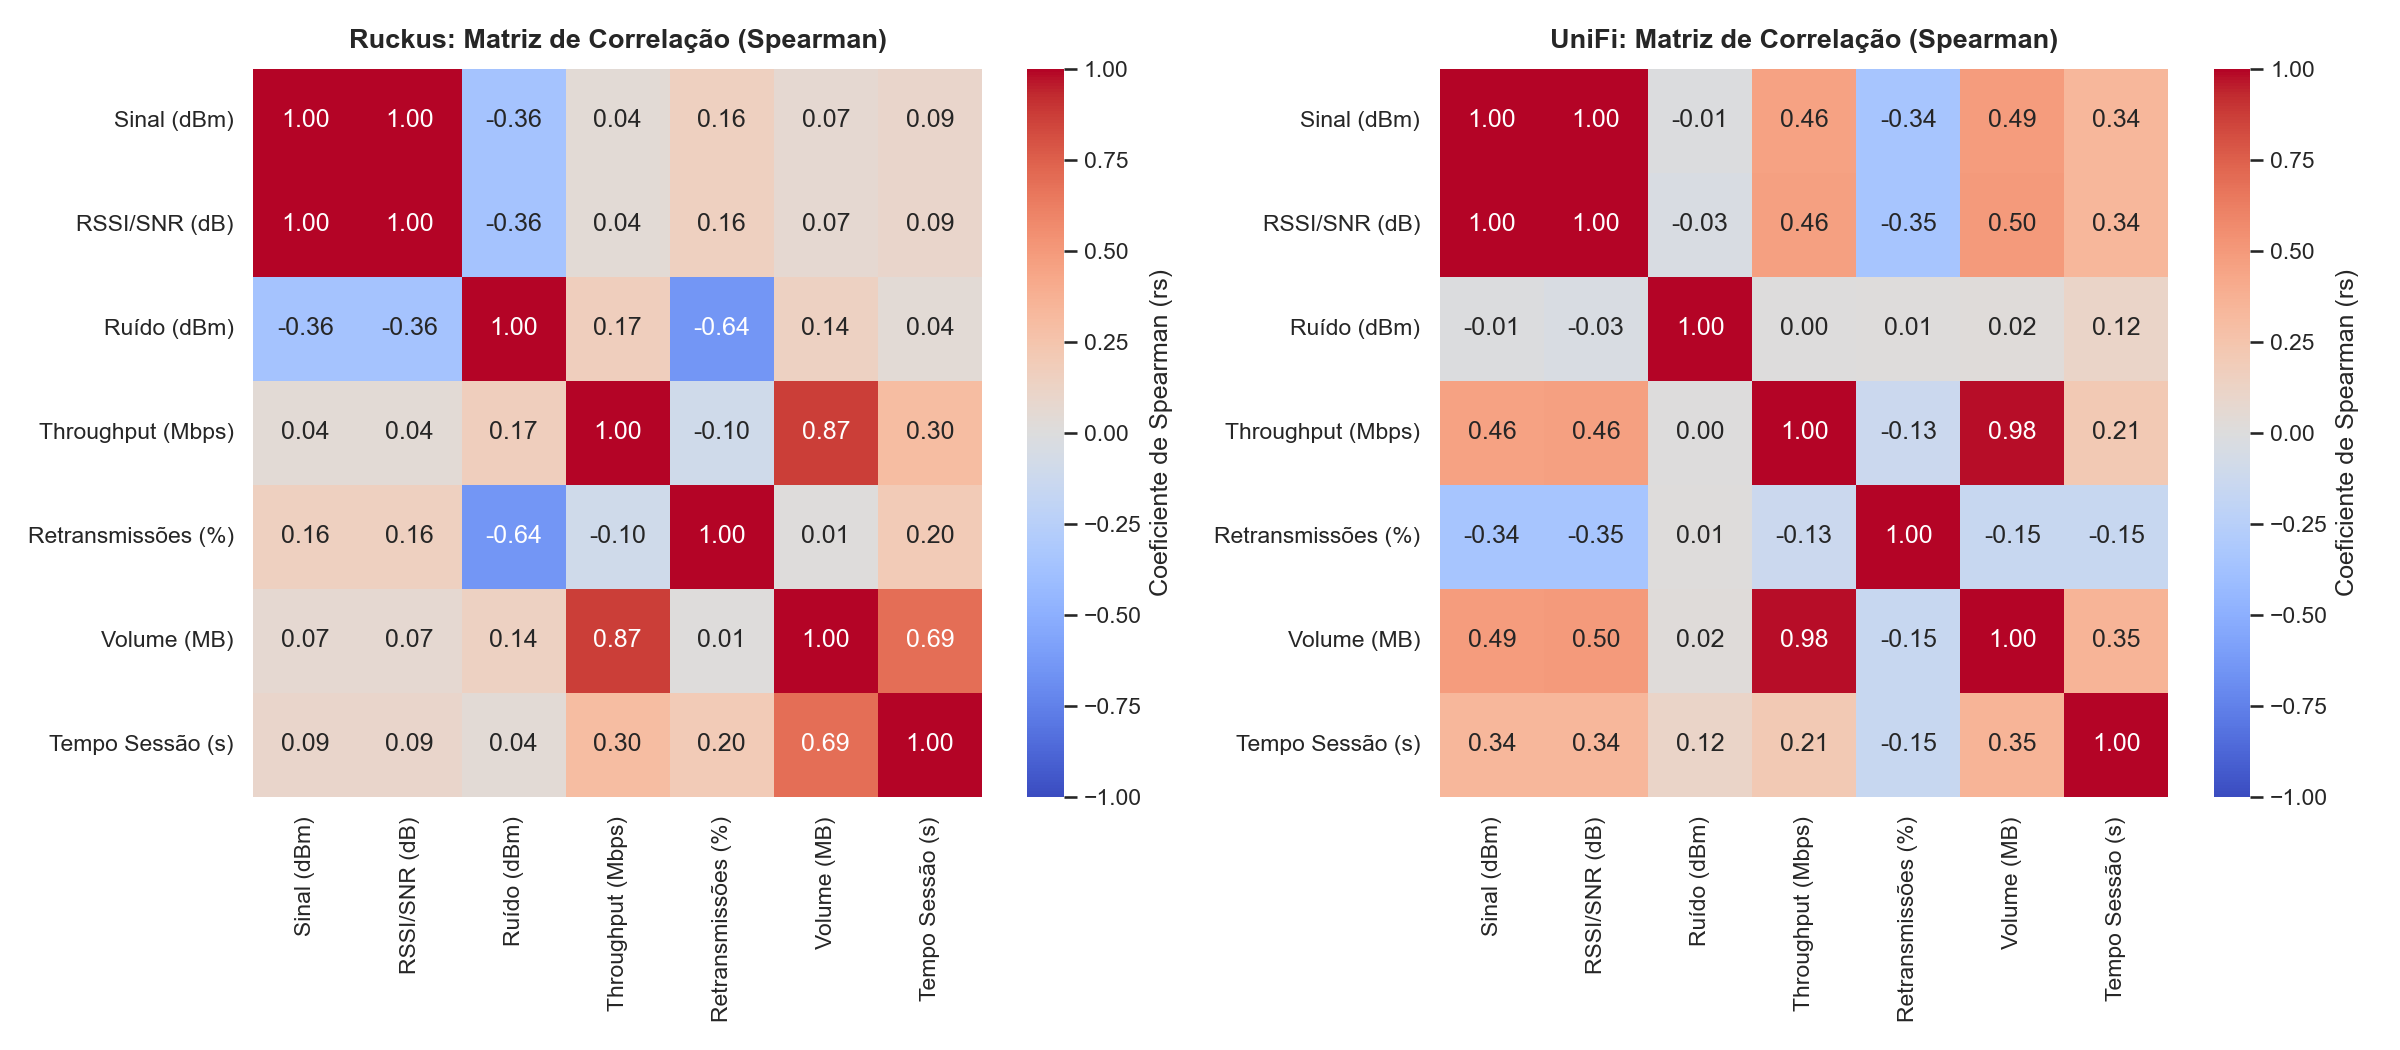
\includegraphics[width=\textwidth,height=0.88\textheight,keepaspectratio]{img/matriz_correlacao_heatmap.png}%
            }
        \end{center}
        \vspace{-0.2cm}
        \centering
        \hyperlink{slide_correlacoes}{\beamerreturnbutton{Voltar}}
    \end{frame}

    \begin{frame}[plain,noframenumbering,label=zoom_jain]
        \begin{center}
            \hyperlink{slide_testes}{%
                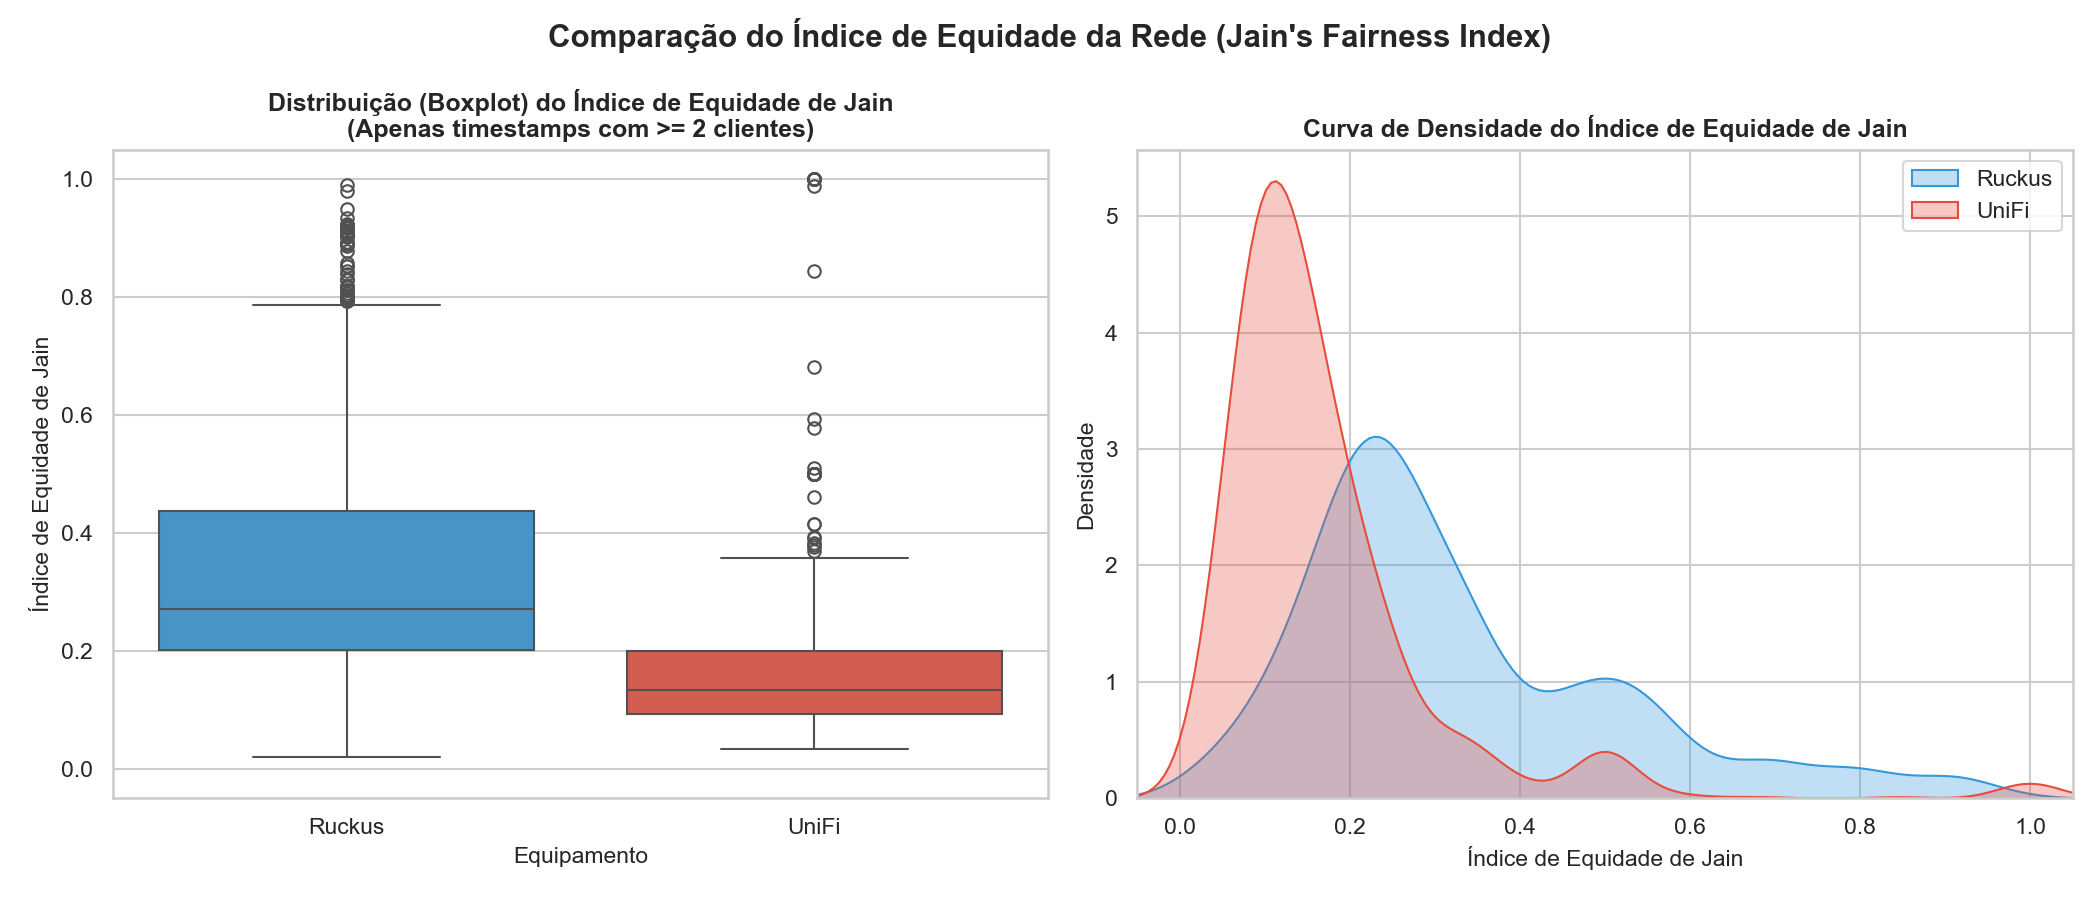
\includegraphics[width=\textwidth,height=0.88\textheight,keepaspectratio]{img/comparativo_equidade.png}%
            }
        \end{center}
        \vspace{-0.2cm}
        \centering
        \hyperlink{slide_testes}{\beamerreturnbutton{Voltar}}
    \end{frame}

\end{document}
